%% LyX 2.0.3 created this file.  For more info, see http://www.lyx.org/.
%% Do not edit unless you really know what you are doing.
\documentclass[french,english]{book}
\usepackage[T1]{fontenc}
\usepackage[latin9]{inputenc}
\usepackage[paperwidth=21cm,paperheight=29cm]{geometry}
\geometry{verbose,tmargin=6cm,bmargin=6cm,lmargin=4.75cm,rmargin=4.75cm}
\pagestyle{plain}
\setcounter{tocdepth}{3}
\usepackage{textcomp}
\usepackage{amssymb}
\usepackage{graphicx}

\makeatletter

%%%%%%%%%%%%%%%%%%%%%%%%%%%%%% LyX specific LaTeX commands.
%% Special footnote code from the package 'stblftnt.sty'
%% Author: Robin Fairbairns -- Last revised Dec 13 1996
\let\SF@@footnote\footnote
\def\footnote{\ifx\protect\@typeset@protect
    \expandafter\SF@@footnote
  \else
    \expandafter\SF@gobble@opt
  \fi
}
\expandafter\def\csname SF@gobble@opt \endcsname{\@ifnextchar[%]
  \SF@gobble@twobracket
  \@gobble
}
\edef\SF@gobble@opt{\noexpand\protect
  \expandafter\noexpand\csname SF@gobble@opt \endcsname}
\def\SF@gobble@twobracket[#1]#2{}
%% Because html converters don't know tabularnewline
\providecommand{\tabularnewline}{\\}

%%%%%%%%%%%%%%%%%%%%%%%%%%%%%% User specified LaTeX commands.
\usepackage{wrapfig}
 \setlength{\intextsep}{0cm plus1cm minus1cm}
\newcommand{\menuitem}[1]{\textbf{\emph{#1}}}

\makeatother

\usepackage{babel}
\addto\extrasfrench{%
   \providecommand{\og}{\leavevmode\flqq~}%
   \providecommand{\fg}{\ifdim\lastskip>\z@\unskip\fi~\frqq}%
}

\begin{document}
\begin{flushleft}
\thispagestyle{empty}
\par\end{flushleft}

\vspace{0.5in}


\begin{center}
{\Huge expEYES}
\par\end{center}{\Huge \par}

\begin{center}
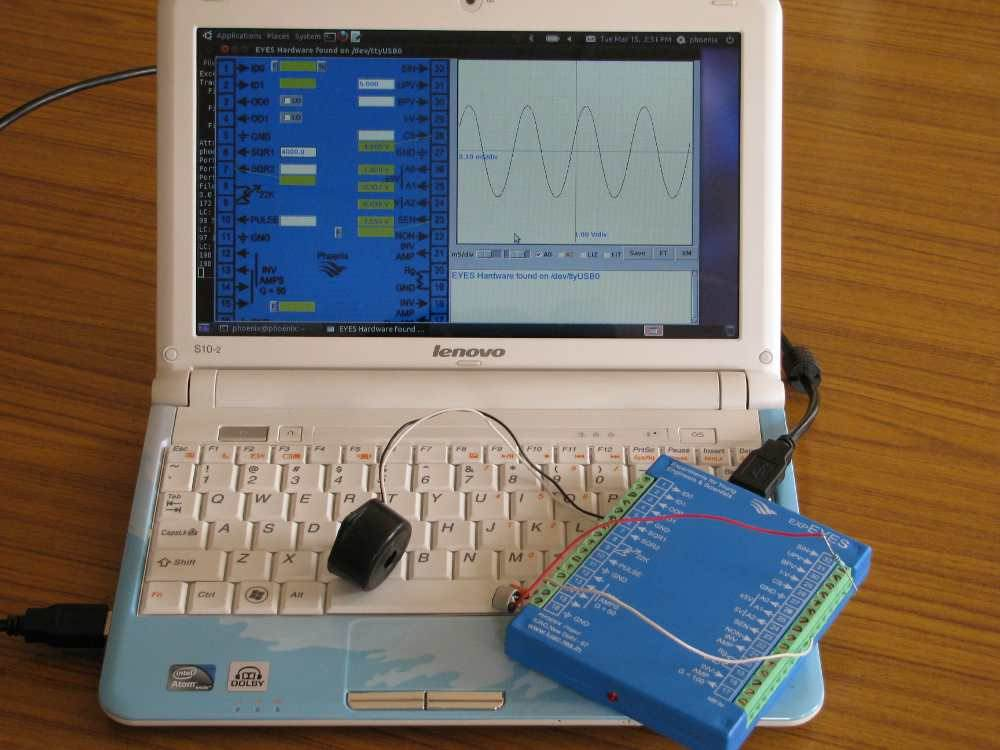
\includegraphics[width=8cm]{pics/eyes}
\par\end{center}

\begin{center}
{\LARGE Experiments for}\\
{\LARGE{} Young Engineers and Scientists}
\par\end{center}{\LARGE \par}

\begin{center}
website : expeyes.in
\par\end{center}

\vspace{0.5in}


\begin{center}
{\large User Manual (ver.2, Apr-2011)}
\par\end{center}{\large \par}

\begin{center}
with 50 Science Experiments
\par\end{center}

\vspace{0.25in}


\begin{center}
PHOENIX Project\\
Inter-University Accelerator Centre\\
(A Research Centre of UGC)\\
New Delhi 110 067\\
www.iuac.res.in
\par\end{center}

\newpage{}

Preface

The PHOENIX (Physics with Home-made Equipment \& Innovative Experiments)
project was started in 2004 by Inter-University Accelerator Centre
with the objective of improving the science education at Indian Universities.
Development of low cost laboratory equipment and training teachers
are the two major activities under this project. The first product
was a general purpose interface, was also called Phoenix, followed
by instruments like Geiger-Muller counter, Alpha spectrometer etc.
The power of personal computers have been utilized for performing
measurements and data analysis.

The new product, expEYES (Experiments for Young Engineers \& Scientists),
is meant to be a tool for learning by exploration, suitable for high
school classes and above. An attempt is made to strike a balance between
open ended experiments mostly meant for exploration and the conventional
ones with some specific objective. We have tried optimizing the design
to be simple, flexible, rugged and above all low cost. There is no
need of a separate power supply since it runs on the 5 volt USB power,
taking care of the long power failures common in many places. The
low price makes it affordable to individuals and we hope to see students
performing experiments outside the four walls of the laboratory, that
closes when the bell rings.

Design of hardware developed is open and the software is released
under GNU General Public License. The project has progressed due to
the active participation and contributions from the user community
and many other persons outside IUAC. We thank them all and also expect
their continued cooperation. We are grateful to Prof. G.K.Mehta for
suggesting corrections to this document. This is distributed under
GNU Free Documentation License. More details and updated versions
of this document are available on the website\textit{expeyes.in}

~

Ajith Kumar B.P.

V V V Satyanarayana

Jimson Sacharias

Deepak Munda

S. Venkataramanan

\newpage{}

\tableofcontents{}

\newpage{}


\chapter{Getting Started}


\section{Introduction}

Performance of a student is often measured by the ability to memorize
than the real understanding. As a result, most of them fail to apply
what they learn in the classroom to things they encounter in their
daily life. To some extent this can be corrected by learning based
on exploration and experimenting. Experiments generally involve measuring
and controlling physical parameters like temperature, pressure, velocity,
acceleration, force, voltage, current etc. If the measured physical
property is changing rapidly, the measurements need to be automated
and a computer becomes a useful tool. For example, understanding the
variation of AC mains voltage with time requires measuring it after
every millisecond.

The ability to perform experiments with reasonable accuracy, opens
up an entirely new path for learning science. Students can compare
the experimental data with mathematical models and examine the fundamental
laws governing various phenomena. Research scientists formulate hypotheses,
design and perform experiments, analyze the data to check whether
they agree with the theory. The objective of PHOENIX (Physics with
Home-made Equipment and Innovative Experiments) project is to provide
the same facilities on a smaller scale to the students. It also enables
the users to develop new experiments without getting into the details
of electronics or computer programming. There are several equipment
and experiments developed so far. This document describes some experiments
that can be done with the interface named\textit{expEYES}.


\section{The equipment}

ExpEYES is interfaced and powered by the USB port of the computer.
For connecting external signals, it has 32 Input/Output terminals,
arranged on both sides, as shown in figure\ref{fig:ExpEYES top panel}.
It can monitor and control the voltages at the terminals. In order
to measure other parameters (like temperature, pressure etc.), we
need to convert them in to electrical signals by using appropriate
sensor elements. Even though our primary objective is to do experiments,
you are advised to read through the brief description of the equipment
given below.

\textit{IMPORTANT : The external voltages connected to expEYES must
be within$\pm5V$ range.}

\begin{figure}
\begin{centering}
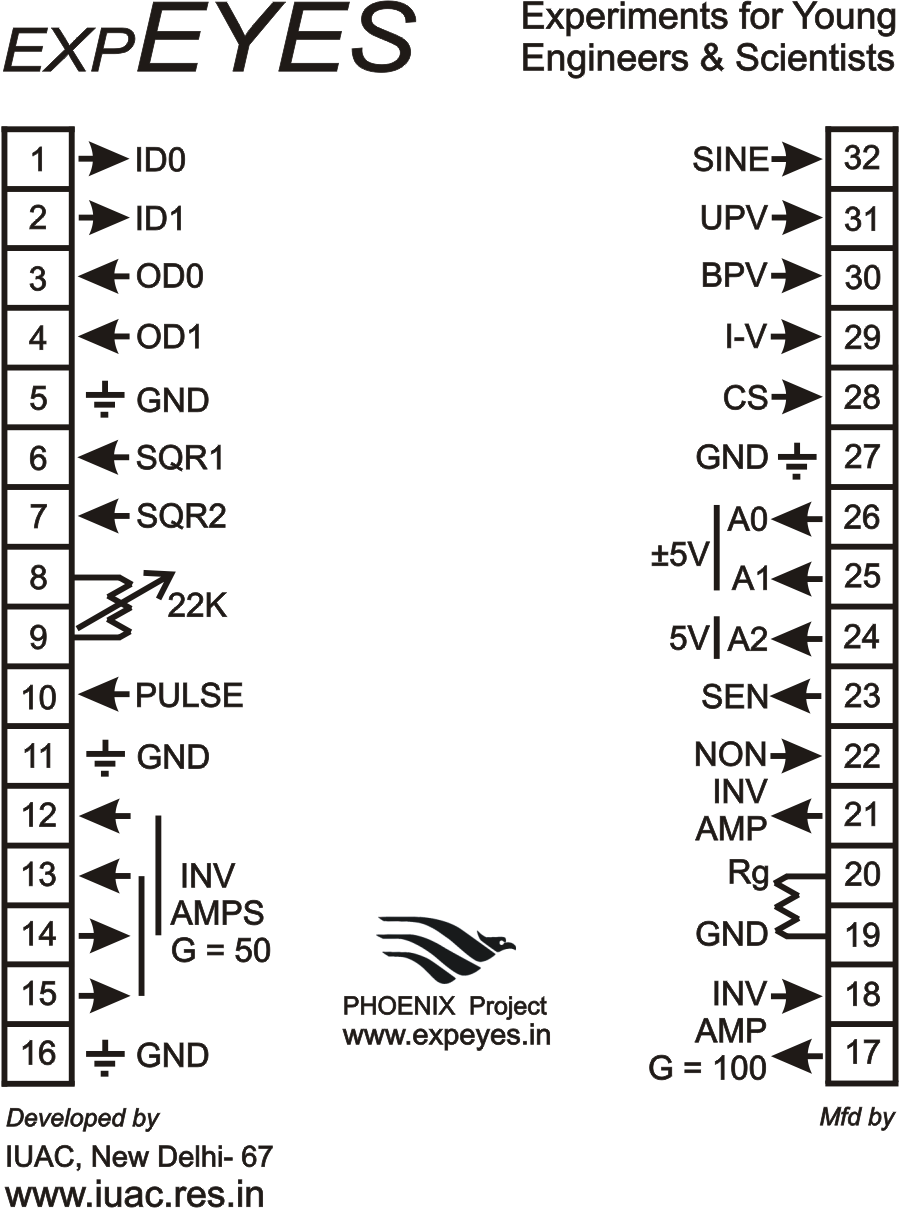
\includegraphics[width=10cm]{pics/top-panel}
\par\end{centering}

\caption{The ExpEYES top panel showing the external connections on both sides.
The arrows indicates the direction of the signals.\label{fig:ExpEYES top panel}.}
\end{figure}



\subsection{External connections}

The external connections can be grouped according to their functions.


\subsubsection*{Digital Inputs (ID0 and ID1)}

Software can read the voltage level applied to them. Any voltage less
than .8~V is treated as 0 (LOW) and anything higher than 2~V is
treated as 1 (HIGH). If the voltage input is changing between HIGH
and LOW, these terminal can measure the frequency and duty-cycle of
the connected signal. ExpEYES is capable of measuring time interval
between voltage transitions on these pins with microsecond resolution.


\subsubsection*{Digital Outputs (OD0 and OD1)}

Using software, we can make the voltage at these terminals 0 or 5~V.
OD0 is transistor buffered and can drive up to 100~mA current. OD1
can only drive only up to 5~mA.


\subsubsection*{Signal Generators}


\paragraph*{SINE}

Fixed frequency sine wave generator, frequency is around 100~Hz.
Bipolar signal output with an amplitude of around 4~V.


\paragraph*{SQR1}

Can generate a square wave, swings from 0 to 5~V. Frequency is programmable
from 15~Hz to 1~MHz. All intermediate values of frequency are not
possible.


\paragraph*{SQR2}

Can generate a square wave, swinging from 0 to 5~V. Frequency can
be set anywhere between 0.7~Hz and 90~kHz. The oscillator requires
an external variable resistor, 22~k$\Omega$, for its operation.
The frequency range is controlled by software and frequency tuning
within the selected range is done by adjusting the resistance. The
frequency ranges are < 25~Hz, 25 to 1~kHz, 1~kHz to 10~kHz and
10~kHz to 90~kHz. Entering a frequency in a particular range selects
that range. The variable resistor is then adjusted to obtain the desired
frequency. The actual value of the frequency is measured and displayed
during adjustment.


\paragraph*{PULSE}

Output frequency is 488~Hz. Duty cycle can be programmed from 0 to
100~\% in 255 steps. This terminal can be configured to generate
a Square wave, like SQR1. This feature is used by the program demonstrating
interference of sound.


\subsubsection*{Analog Voltage Inputs}


\paragraph*{A0 and A1}

Can measure voltage within the$\pm5\, V$ range. The resolution of
ADC used is 12~bits. Voltage at these terminals can be displayed
as a function of time, giving the functionality of a low frequency
two channel oscilloscope.


\paragraph*{A2}

For voltage measurement. Input must be within the 0 to 5~V range.
Resolution is 12~bits. Voltage can be displayed as a function of
time using software.


\subsubsection*{Analog Voltage Outputs}


\paragraph*{BPV}

Bipolar voltage output. Can be programmed to any value between -5~V
to +5~V. The resolution is 12 bit, implies a minimum voltage step
of around 2.5~mV.


\paragraph*{UPV}

Unipolar voltage output. Can be programmed between 0 to +5~V. Cannot
be used along with the current source output CS, since they share
the same DAC output.


\paragraph*{IV}

This is just the output BPV coming out through a 1$k\Omega$ resistor.
Used for doing I-V characteristic.


\subsubsection*{Constant Current Source (CS)}

Programmable to any value from 0.05 to 2.0~mA. The load resistor
should be chosen such that the the product$IR$ is less than 2~V.
Remember that CS and UPV shares the same DAC output.


\subsubsection*{Inverting Amplifiers}

There are three inverting amplifiers, implemented using TL084 op-amps,
denoted below using their input and output terminal numbers.


\paragraph*{15$\Rightarrow$13}

Input at terminal 15 and output at 13. Default Gain=50. The gain can
be reduced by feeding the input through a series resistor. The gain
is be governed by$G=\frac{R_{f}}{(R_{ext}+1000)}$ where the internal$R_{f}=50000\,\Omega$.
The external series resistor is$R_{ext}$.


\paragraph*{14$\Rightarrow$12}

Input at terminal 14 and output at 12. Similar to the one mentioned
above.


\paragraph*{17$\Rightarrow$18}

Input at 17 and output at 18. Default Gain=100. The gain can be reduced
by feeding the input through a series resistor. The gain is be governed
by$G=\frac{R_{f}}{(R_{ext}+100)}$ where the internal$R_{f}=10000\,\Omega$
and the external series resistor is$R_{ext}$.


\subsubsection*{Non-Inverting Amplifier}

The input is at 21 and output at 22. The gain is decided by an external
resistor$R_{g}$ connected between 19 and 20 and is given by$Gain=1+10000/R_{g}$.
This amplifier is implemented using OP27 IC and has an offset voltage
of around$30\,\mu V$.


\subsubsection*{Sensor Input (SEN)}

For connecting any sensor whose resistance varies with the measured
parameter. When used with the photo-transistor. connect collector
to this, and emitter to Ground. Capable of measuring the voltage and
frequency.


\subsubsection*{Frequency Counters}

The terminal 15 can measure the frequency of a bipolar signal (that
goes to both negative and posiive values). The minimum measurable
amplitude is 100~mV and the maximum is 5~V.

ID0, ID1 and SEN are capable of measuring the frequency of signals
swinging from 0 to 5~V.


\section{Software Installation}

ExpEYES can run on any computer having a Python Interpreter and a
Python module to access the Serial port. The USB interface is handled
by the device driver programs that presents the USB port as an RS232
port to the application programs. The communication with expEYES is
done using a library written in Python language. Programs with GUI
have been written for many experiments. There are many ways to get
the software running:


\subsubsection*{The expEYES Live CD}

The easiest way to get started is to boot your PC with the Phoenix
Live-CD. From the PC BIOS, make the CD drive as the first boot device,
insert the live CD and reboot the PC. A desktop will appear and you
can start expEYES from the menu\textbf{Applications~->~Science}.
The expEYES live CD is made from GNU/Linux distribution Ubuntu 10.10.


\subsubsection*{Installing on Debian or Ubuntu GNU/Linux distributions}

Install python-imaging-tk from the repository of the distribution
you are running. Download\textbf{expeyes.deb} from\textbf{http://expeyes.in}
and install it. Also install python-scipy and grace (a 2D plotting
program) for full functionality.


\subsubsection*{For other GNU/Linux distributions}

Download\textbf{expeyes.tgz} from\textbf{http://expeyes.in} and follow
the instructions in the README file. It is important to give read/write
permissions for all users on the USB port where expEYES is connected.


\subsubsection*{On MSWindows}

Even though expEYES is Free Software and it developed using Free and
Open software, it runs on non-free platforms also. To install it on
MS windows, you need the following files (given on the CD)
\begin{enumerate}
\item CDM20814\_Setup.exe
\item python-2.6.6.msi
\item pyserial-2.5.win32.exe
\item PIL-1.1.7.win32-py2.6.exe
\item numpy-1.6.0b2-win32-superpack-python2.6.exe
\item scipy-0.9.0-win32-superpack-python2.6.exe
\item expeyes.zip
\end{enumerate}
Unzip the file\textbf{expeyes.zip}, and double click on\textbf{explore.py}
inside the newly created directory named EYES.

If you have expEYES liveCD, browse inside the directory named WINEYES.
All the files mentioned above are inside that directory. Double click
on them in the order mentioned above to install them. The XmGrace
plotting utility is not available under MSwindows. Fourier transform
output will be saved to disk in text format.


\section{The main GUI program}

Start Applications->Science->expEYES from the menu. It will show a
graphics window as shown in figure\ref{fig:Explorer screenshot},
and is briefly explained below.
\begin{itemize}
\item Clicking on the boxes showing the terminal numbers will display help
messages.
\item Right Clicking on the left panel produces a pop-up menu of applications.
\item The status of Digital Inputs decides the colour of the display area
against them. Pale green indicates High and Gray indicates Low. When
the input voltage swings from 0 to 5 volts, this field blinks.
\item The display field against T15 may blink if an AC signal is given there.
\item The Frequency display field of SEN may blink if the input is varying
between 0 and 5 volts. This will happen if the connected resistance
is varying.
\item The Buttons marked 'F' may be used for measuring the frequency, while
the display fields are blinking.
\item The values of output signals can be set by entering them in the nearby
text box. Voltage, current, frequency and duty-cycle are set like
this. Press <Enter> to set the entered value. If successful, the display
will show a decimal point.
\item SQR2 require an external resistor to function, we use a 22k$\Omega$
variable resistor. The actual frequency is displayed just below the
text field, where you set the frequency.
\item State of Digital Outputs, OD0 and OD1, can be changed by using the
Check Buttons.
\item The voltages at the input terminals 23,24,25 and 26 are displayed
continuously against them.
\end{itemize}
The GUI is made using a photograph of the device. Control and monitor
widgets are placed on the photograph at appropriate places. Right
click on the panel to get a pop-up menu of application programs for
various experiments.


\subsubsection*{The Plot Window}

The plot window on the right side works like a low frequency oscilloscope.
The maximum sampling rate is 100~kHz only. You can digitise sinewaves
upto 20~kHz while using only one channel and upto 10~kHz when both
are enabled. The following controls are available.
\begin{itemize}
\item Horizontal scale Slider (ms/Sec). Set this to the minimum value and
increase to view more number of cycles on the screen.
\item Channel selection Checkboxes for A0 and A1.
\item LIZ checkbox to make a Lissajous figure using A0 and A1 inputs.
\item FIT checkbox to enable calculating amplitude, frequency and phase
by fitting the data using the equation$V=V_{0}\sin\left(\omega t+\theta\right)+C$
. The RMS value of the voltage and frequency are displayed. When both
the channels are selected, the phase difference is diplayed.
\item SAVE button to save the data to\textit{explore.dat} as two column
text.
\item FT to do a Fourier Transform power spectrum of the data from enabled
channels. If Xmgrace and pygrace are installed, a window is opened.
Power spectrum is saved to\textit{exploreFFT.dat} in text form.
\end{itemize}

\section{Basic measurements using expEYES}

\begin{figure}
\begin{centering}
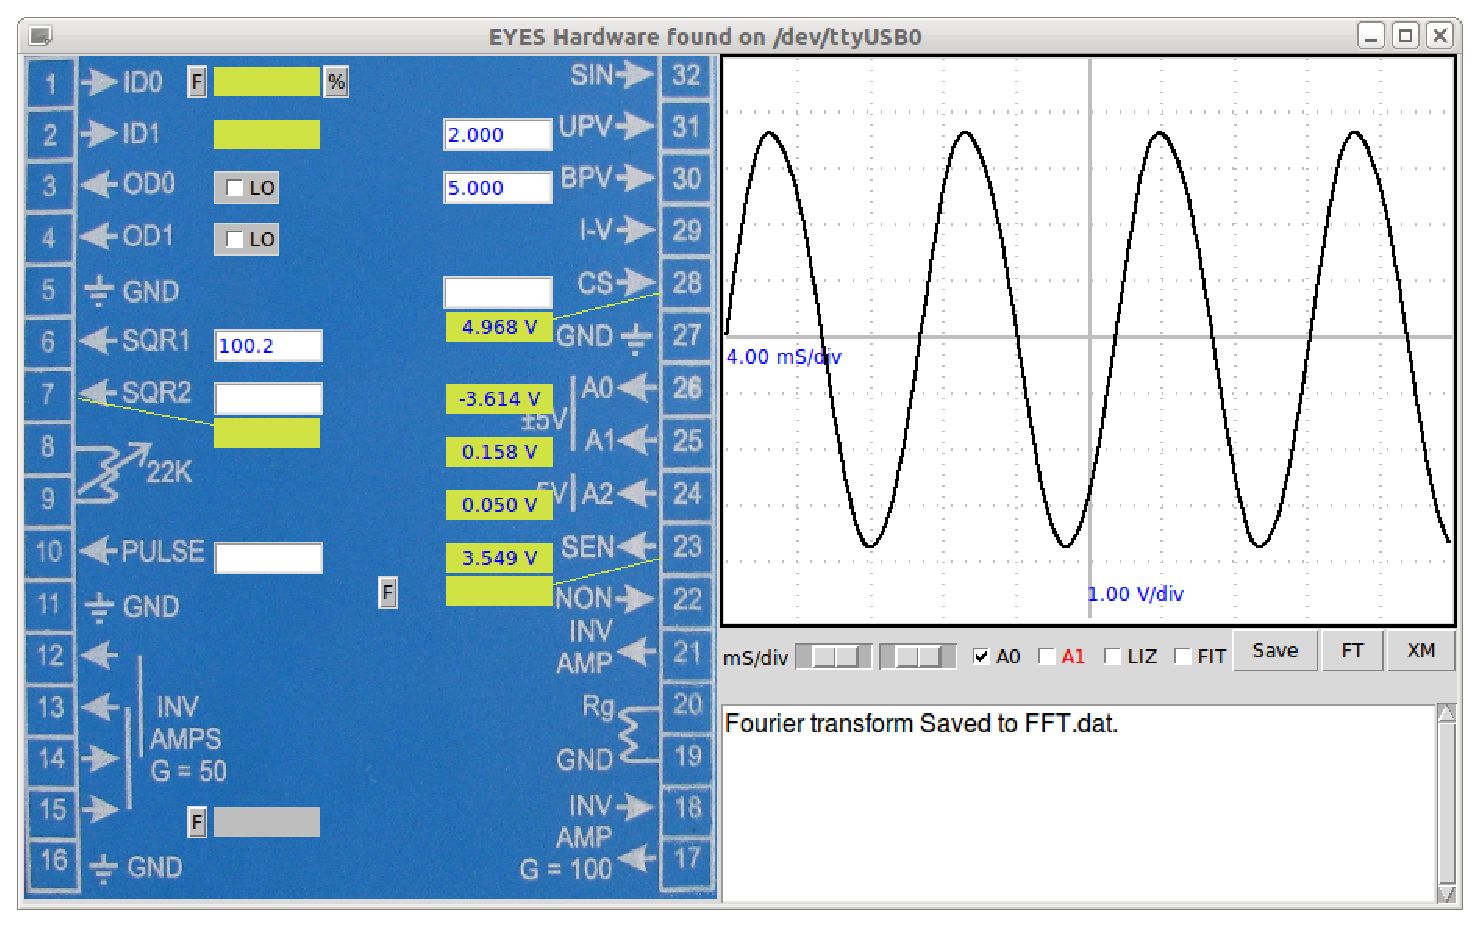
\includegraphics[width=11cm]{pics/explorer}
\par\end{centering}

\caption{Screen shot of Explore program. Arrows indicate the signal direction.
Text fields are used for setting values. Buttons are provided for
frequency measurements.\label{fig:Explorer screenshot}}
\end{figure}


Before proceeding with the experiments, let us do some simple exercises
to become familiar with expEYES. Boot your computer from the LiveCD,
connect expEYES to the USB port and start the expEYES program from
the menu 'Applications->Science'.


\subsection{Generate \& measure voltages}
\begin{itemize}
\item Connect BPV to A0
\item Set BPV to some voltage and observe the reading at A0
\item Try A1 instead of A0
\item Repeat the same by connecting UPV to A2
\end{itemize}

\subsection{Observe voltage waveforms}
\begin{itemize}
\item Connect SQR1 to A0
\item Set SQR1 to 100 Hz
\item Adjust the horizontal scale (ms/Div) to view 4 or 5 cycles of the
square wave
\item Repeat with other frequency values
\item Connect SINE to A1 and watch both traces simultaneously
\item Explore the FIT, XM and FT options.
\end{itemize}

\subsection{Measure frequency}
\begin{itemize}
\item Connect SQR1 to ID0
\item Set SQR1 to 1000
\item Click on the 'F' button of ID0
\item Connect SINE to T15 and measure the frequency.%
\footnote{T15 will not measure the frequency of SQR1 or SQR2 outputs, because
they do not swing below zero.%
}
\end{itemize}

\subsection{Measure duty cycle}
\begin{itemize}
\item Connect PULSE to ID0
\item Also to A0, if you want to watch the waveform.
\item Set PULSE to any value from 0 to 100
\item Click on the '\%' button of ID0, to measure the duty cycle.
\end{itemize}

\subsection{Setting voltage levels}
\begin{itemize}
\item Connect OD0 to ID0
\item Click on the Check button and watch ID0 display color.
\end{itemize}

\section{Experiments}

A science experiment generally involves control and measurement of
various physical parameters like temperature, pressure, voltage, current
etc. The basic expEYES hardware can generate different kinds of electrical
signals and measure electrical signals. For measuring anything other
than voltage, we need to convert it using appropriate sensor elements.
For example a temperature sensor will give a voltage indicating the
temperature. Since experiments in electricity and magnetism does not
require any sensor elements, we have more number of experiments based
on electricity and magnetism.

A GUI program is provided for every experiment given in this manual.
However, it is possible to do the same by writing few lines of code
written in Python language. All the communication to expEYES is done
using a Python library called\textit{eyes.py}. Python libraries are
used for data analysis. If you are interested in developing new experiments
based on expEYES, it would be a good idea to learn Python programming
language. Almost every experiment can be extended in several ways
and some hints are given in this direction.

The following chapters describe experiments from different topics
like electricity, magnetism, electronics, sound, heat, etc. Since
the expEYES kit is meant for self learning, we have included some
very trivial experiments in the beginning.


\chapter{Electricity}

We start with the trivial task of measuring the voltage of a battery.
Current and resistance are introduced next, followed by resistances
changing with temperature and light. The concept of Alternating Current
is introduced by plotting the voltage as a function of time. The behavior
of circuit elements like capacitors and inductors in AC and DC circuits
are explored, by measuring parameters like amplitude, frequency and
phase. The transient response of a resistor and capacitor in series
is used for measuring the capacitance. Inductance also is measured
in the same manner. The effect of ferromagnetic materials inside an
inductor in examined.

The Fourier analysis of square wave is done to study the harmonics.
Integration and differentiation of a square wave using RC circuits
also is explored.

\newpage{}


\section{Measuring voltage\label{sec:Measuring-Voltage-*}}


\subsection*{Objective}

Learn to measure voltage using expEYES and get some idea about the
concept of Electrical Ground.


\subsection*{Equipment}

\begin{figure}
\begin{centering}
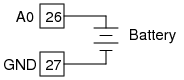
\includegraphics[height=2cm]{schematics/cell-volatge}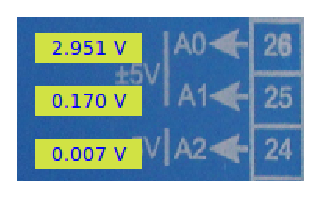
\includegraphics[height=2cm]{pics/drycell-voltage}
\par\end{centering}

\caption{Measuring the voltage of a battery\label{fig:Measuring-drycells}}


\end{figure}

\begin{itemize}
\item 1.5 Volts dry cells
\item Battery holder with two connecting wires.
\end{itemize}

\subsection*{Procedure}
\begin{itemize}
\item Connect Negative terminal of the battery to Ground.
\item Positive terminal of the cell to A0.
\end{itemize}

\subsection*{Observation}

Voltage will be displayed on the left side of A0, as shown in figure\ref{fig:Measuring-drycells}.


\subsection*{Discussion}

We are measuring the potential difference between two points. One
of them can be treated as at zero or Ground potential. The voltage
measuring points of expEYES measure the voltage with respect to the
terminals marked GND. We have connected the negative terminal of the
cell to Ground. The positive terminal is at +3 volts with respect
to the negative terminal.

Repeat the experiment by connecting the positive terminal of the cell
to GND and the negative to A0. The voltage will be shown as negative.\textit{Will
it show correct voltage if Ground is not connected ?}

\newpage{}


\section{Voltage, current \& resistance}


\subsection*{Objective}

Learn about Current, Resistance and Ohm's law. Plot I-V curve of a
resistor.


\subsection*{Theory}

The voltage across a conductor is directly proportional to current
flowing through it. The constant of proportionality is called Resistance.
This is known as Ohm's Law, expressed mathematically as
\[
V\varpropto I\,\,\,;\,\,\,\, V=IR\,\,\,\, or\,\,\, R=\frac{V}{I}
\]



\subsection*{Equipment}

\begin{flushleft}
\begin{figure}
\begin{centering}
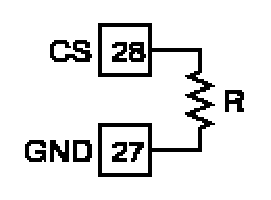
\includegraphics[width=3cm]{schematics/res-measure}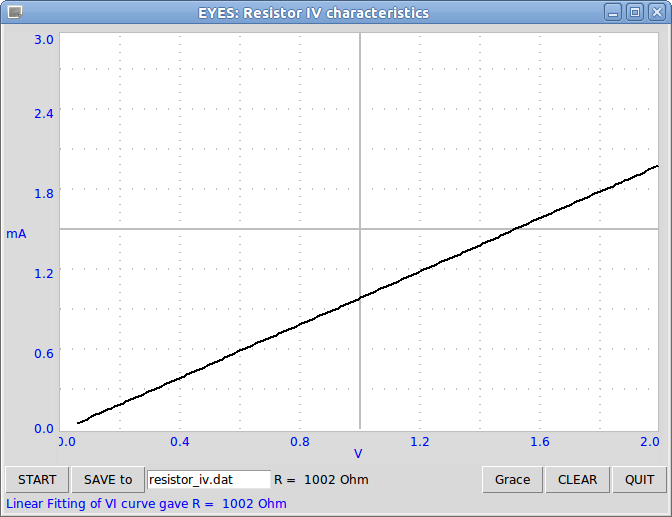
\includegraphics[width=4cm]{pics/resistor_iv}
\par\end{centering}

\caption{IV-characteristic of resistor\label{fig:I-V of -resistor}}
\end{figure}

\par\end{flushleft}
\begin{itemize}
\item A$1\, k\Omega$ resistor
\end{itemize}

\subsection*{Procedure}
\begin{itemize}
\item Connect resistor from CS to Ground.
\item Set the current to 0.5~mA and note down the voltage at CS.
\item Change the current in .5~mA steps. (V should not exceed 2~V at CS)
\item Right click on the Panel. Choose\textit{\menuitem{Resistor IV}} from
the pop-up menu.
\item Draw the graph using\buttonlabel{START} button.
\end{itemize}

\subsection*{Observation}

\begin{tabular}{|c|c|}
\hline 
I~(mA) & V~(volt)\tabularnewline
\hline 
\hline 
0.5 & .508\tabularnewline
\hline 
1.0 & 1.011\tabularnewline
\hline 
1.5 & 1.5.10\tabularnewline
\hline 
\end{tabular}

The current source accuracy is only 1\%, due to the tolerance value
of the resistor used. For applications requiring higher accuracy,
you can calibrate it using a known resistance. The I-V curve is shown
in figure\ref{fig:I-V of -resistor}.


\subsection*{Discussion}

Using expEYES, we can set the current from CS (from 0.05~mA to 2~mA).
The voltage at CS will depend on the resistance connected from the
current source to Ground.%
\footnote{ The voltage across this particular current source should not exceed
2 volts. Choose the load resistor and current values accordingly.%
}

The graph is a straight line since the voltage is directly proportional
to current. The graph will not be a straight line for non-linear elements,
like a diode.\newpage{}


\section{Resistances in series}


\subsection*{Objective}

Finding the effective resistance of a series combination of resistors.


\subsection*{Theory}

For series combination of resistors, total resistance is given by$R=R1+R2+\cdots$


\subsection*{Equipment}
\begin{itemize}
\item $560\,\Omega$ and$1\, k\Omega$ resistors
\end{itemize}

\subsection*{Procedure}

\includegraphics[height=0.8cm]{schematics/res-series}
\begin{itemize}
\item Connect both resistors in series from CS to Ground
\item Set the current to 1 mA and note down the voltage displayed at CS.
\end{itemize}

\subsection*{Observation}

\begin{tabular}{|c|c|}
\hline 
R~($\Omega)$ & V~(volts)\tabularnewline
\hline 
\hline 
560 & .558\tabularnewline
\hline 
1000 & 0.998\tabularnewline
\hline 
1000+560 & 1.556\tabularnewline
\hline 
\end{tabular}

Since the current is same, the total voltage drop gives the effective
resistance. It can be seen that it is the sum of the individual values,
within the measurement error.


\subsection*{Discussion}

Very high resistances ($>10^{9}\Omega$) are often implemented using
series combinations.\newpage{}


\section{Resistances in parallel}


\subsection*{Objective}

Find the effective resistance of parallel combination of resistors.


\subsection*{Theory}

For parallel combination, effective resistance is given by
\[
\frac{1}{R}=\frac{1}{R1}+\frac{1}{R2}+\cdots
\]



\subsection*{Equipment}
\begin{itemize}
\item Two 1$k\Omega$ resistors
\end{itemize}

\subsection*{Procedure}


\includegraphics[height=1cm]{schematics/res-par}
\begin{itemize}
\item Connect$1\, k\Omega$ resistor from CS to Ground.
\item Set the current to 1~mA (0.001~Ampere) and note down the voltage
displayed at CS.
\item Repeat the same with two resistors connected in parallel.
\end{itemize}

\subsection*{Observation}

\begin{tabular}{|c|c|}
\hline 
$R_{connected}(\Omega)$ & $V_{measured}(V)$\tabularnewline
\hline 
\hline 
1000 & 1.008\tabularnewline
\hline 
1000$\parallel$1000 & 0.503\tabularnewline
\hline 
\end{tabular}

Since we know the current, we can calculate the resistance from the
measured voltage. As per the measured voltage the resistance of the
parallel combination is$\frac{0.503\, V}{0.001\, A}=503\,\Omega$


\subsection*{Discussion}

Why one wants to connect resistors in parallel ?

\newpage{}


\section{Measure resistance by comparison\label{sec:Measure-resistance-by}}


\subsection*{Objective}

Learn to apply Ohm's law to find the value of an unknown resistance
by comparing it with a known one.


\subsection*{Theory}

Voltage across a resistor is given by$V=IR$ . If same amount of current
is flowing through two different resistors, the ratio of voltages
will be the same as the ratio of resistances.
\[
I=\frac{V1}{R1}=\frac{V2}{R2}
\]



\subsection*{Equipment}
\begin{itemize}
\item A 1~$k\Omega$ as the reference and another resistors. (some value
from 100~$\Omega$ to 10~$k\Omega$)
\end{itemize}

\subsection*{Procedure}


\includegraphics[height=1cm]{schematics/res-comp}
\begin{itemize}
\item Connect the unknown resistor R from UPV to A2.%
\footnote{We use A2 when the voltage is in the 0 to 5V range.%
}
\item Connect 1~$k\Omega$ (R2) from A2 to Ground.
\item Set UPV to 4 volts.
\item Measure voltage at A2.
\end{itemize}

\subsection*{Observation}

Voltage at A2 = 1.244, implies voltage across the unknown resistor
is$4-1.244=2.756$

Current$I=\frac{1.244}{1000}=1.244mA$

Unknown resistor value =$\frac{2.756}{1.244}=2.215\, k\Omega$


\subsection*{Discussion}

What is the limitation of this method ? How do we choose the reference
resistor ? suppose the unknown value is in Mega Ohms, what will be
the voltage drop across a$1k\Omega$ reference resistor ? Our voltage
measurement is having a resolution of$\frac{1}{4095}$.

We will use this method later to measure the resistance of solutions.

\newpage{}


\section{Voltage of a lemon cell}


\subsection*{Objective}

Make a voltage source. Learn about current capability. Concept of
internal resistance.


\subsection*{Equipment}

\begin{figure}
\begin{centering}
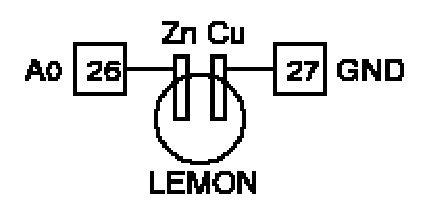
\includegraphics[width=4cm]{schematics/lemon-cell}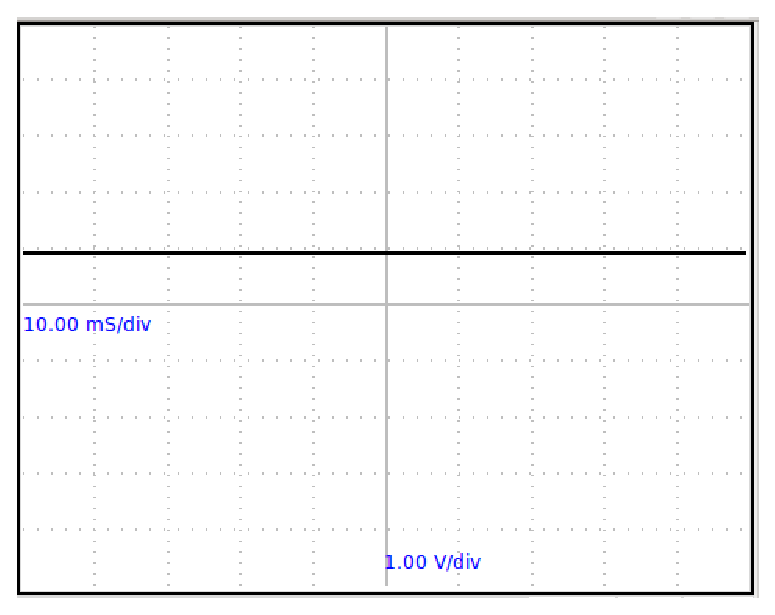
\includegraphics[width=4.6cm]{pics/lemoncellDC}
\par\end{centering}

\caption{(a)Copper and Zinc plates inserted into a Lemon. (b) The DC voltage
output from the cell.\label{fig:lemoncell}}


\end{figure}

\begin{itemize}
\item Ripe Lemon (or some acid), thin Zinc and Copper plates.
\item A 1~$k\Omega$ resistor.
\end{itemize}

\subsection*{Procedure}
\begin{itemize}
\item Insert the zinc and copper plates into the lemon.
\item Connect one plate to ground and another to A0, using two wires.
\item Connect the resistor from A0 to ground.
\end{itemize}

\subsection*{Observation}

Voltage across the Copper and Zinc terminals will be nearly .9 volts.
Connecting the resistor reduces it to .33 volts.

What is the internal resistance of the cell ?


\subsection*{Discussion}

When connected, current will start flowing through the resistor. But
why the voltage is going down ?

It does not happen with a new dry-cell. Why ?

Current is the flow of charges and it has to complete the path. That
means, current has to flow through the cell also. Depending on the
internal resistance of the cell, part of the voltage gets droped inside
the cell itself.

An ideal voltage source should have zero internal resistance.\newpage{}


\section{Voltage changing with time}


\subsection*{Objective}

Introduce the concept of time dependent voltages, using a V(t) graph.


\subsection*{Equipment}

\begin{figure}
\begin{centering}
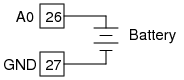
\includegraphics[width=4cm]{schematics/cell-volatge}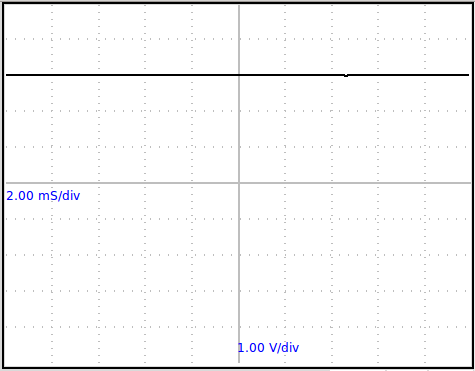
\includegraphics[width=4cm]{pics/dcvoltage}
\par\end{centering}

\caption{Plotting DC voltage with Time\label{fig:Graph-of-DC}}
\end{figure}

\begin{itemize}
\item 1.5 Volts dry cells
\item Battery holder with leads.
\end{itemize}

\subsection*{Procedure}
\begin{itemize}
\item Connect Negative of the dry cell to Ground.
\item Positive terminal of the cell to A0.
\item Observe the graph on the right side window.
\end{itemize}

\subsection*{Observation}
\begin{itemize}
\item A horizontal line appears on the Graph, Time on x-axis and voltage
on y-axis.
\end{itemize}

\subsection*{Discussion}

Voltage is constant in time. A cell is a source of Direct Current
(DC). Another type of current is called Alternating Current or AC,
which changes the magnitude and direction with time.

\newpage{}


\section{Alternating current (AC)}


\subsection*{Objective}

Learn about AC, using graphs. Get familiar with the sinusoidal voltage
waveform.


\subsection*{Equipment}
\begin{itemize}
\item A piece of wire.
\end{itemize}

\subsection*{Procedure}
\begin{itemize}
\item Connect SINE to A0.
\item Adjust the horizontal scale to view 4 to 5 cycles.
\item Enable the Checkbox 'FIT'.
\end{itemize}

\subsection*{Observation}

\begin{figure}
\begin{centering}
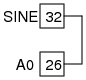
\includegraphics[width=2cm]{schematics/sine-a0}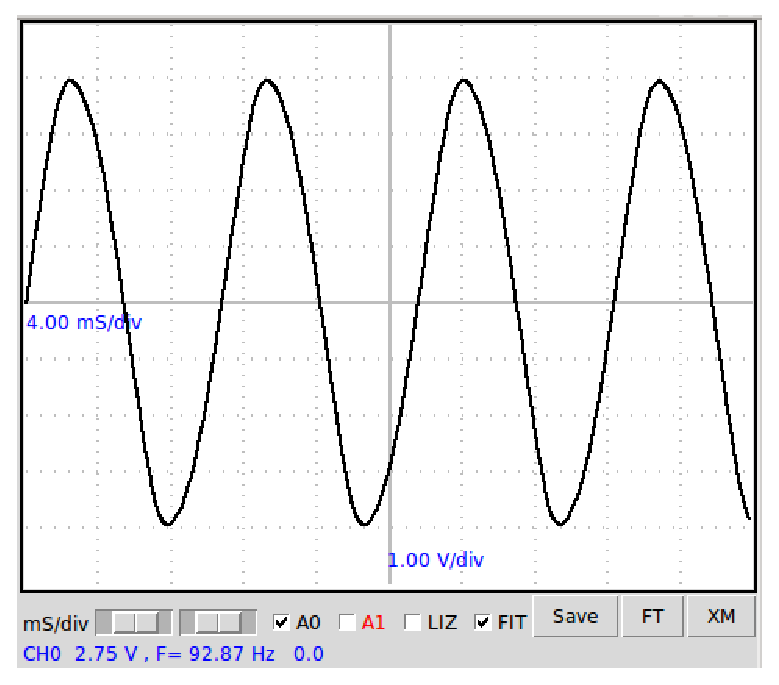
\includegraphics[width=4cm]{pics/sinewave90hz}
\par\end{centering}

\caption{AC voltage waveform from SINE\label{fig:Sinewave}}
\end{figure}

\begin{itemize}
\item The waveform is shown in the figure\ref{fig:Sinewave}. Enable the
'FIT' option to calculate the amplitude and frequency by fitting the
data with the equation$V=V_{0}\sin(2\pi ft+\theta)$ , where$V_{0}$
is the amplitude and$f$~is the frequency.
\end{itemize}

\subsection*{Discussion}

The voltage is changing with time. It goes to both negative and positive.
One full cycle takes around 12 milli seconds, ie. around 90 cycles
per second or 90 Hertz. This voltage waveform is generated by using
electronic circuits.%
\footnote{The frequency of the SIN output is around 90 Hz. It's variation is
due to the 20\% tolerance of the capacitors deciding the frequency.%
}

The AC mains supply coming to our houses has a frequency of 50 Hz.

What is the significance of$\theta$ in the equation above ?

\newpage{}


\section{AC Powerline pickup}


\subsection*{Objective}

Learn about the AC mains supply. Explore the phenomenon of propagation
of AC through free space.


\subsection*{Equipment}
\begin{itemize}
\item A long piece of wire.
\end{itemize}

\subsection*{Procedure}
\begin{itemize}
\item Connect one end of the wire to A0.
\item Take the other end near the power line (never touch the line) and
change the orientation of the wire until you get a good signal on
the screen.
\item Adjust the horizontal scale to 10 milliseconds per division.
\item Enable the Checkbox 'FIT'.
\end{itemize}

\subsection*{Observation}

\begin{figure}
\begin{centering}
\includegraphics[width=4cm]{schematics/pickup}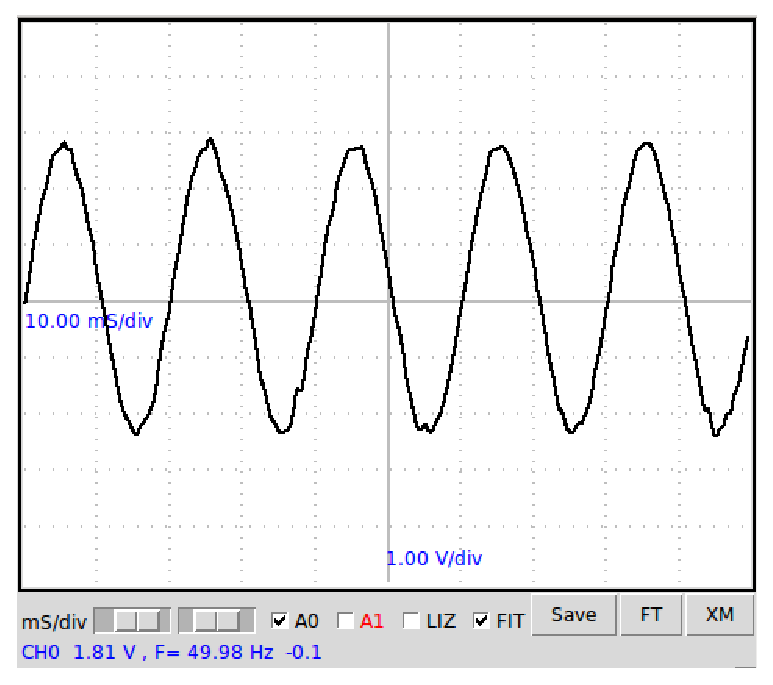
\includegraphics[width=5cm]{pics/sinewave50hz}
\par\end{centering}

\caption{Power line pickup\label{fig:Power-line-pickup}}
\end{figure}


The observed waveform is shown in figure\ref{fig:Power-line-pickup}.
The frequency calculated by fitting the data is 49.65 Hz


\subsection*{Discussion}

Without making any connection, how we are getting the AC voltage from
the mains supply ? Do this experiment with a laptop computer staying
far away from mains supply lines.

Is it similar to the radiation from a cell phone ?

Why the frequency is differing from 50 Hz ?

We are watching the voltage picked up by the wire, it acts as an antenna
and receives the 50 Hz radiation from the power line. Touching the
floating end of the wire increases the pickup, you are becoming part
of the antenna. The frequency$f$ is calculated by fitting the collected
data with the equation$V=V_{0}\sin(2\pi ft+\theta)$.

Try measuring during the daytime and at midnight to compare the measured
frequecies. It depends on the total load on the grid. If the power
distribution system is really good, the frequency will remain constant.

\newpage{}


\section{DC \& AC components of a time dependent voltage\label{sec:DC-&-AC}}


\subsection*{Objective}

Learn about the AC and DC components of a time dependent voltage.
Separating AC and DC using a capacitor.


\subsection*{Equipment}

\begin{figure}
\begin{centering}
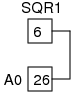
\includegraphics[width=2cm]{schematics/sqr-a0}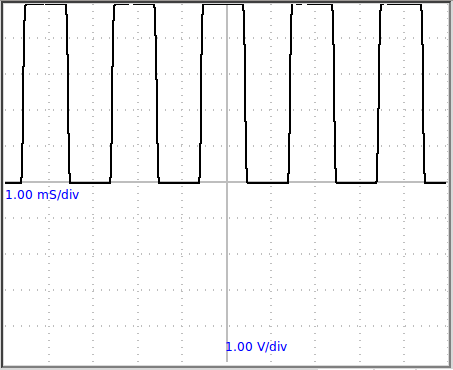
\includegraphics[width=3.3cm]{pics/sqrwave2}\includegraphics[width=2.5cm]{schematics/ac-dc}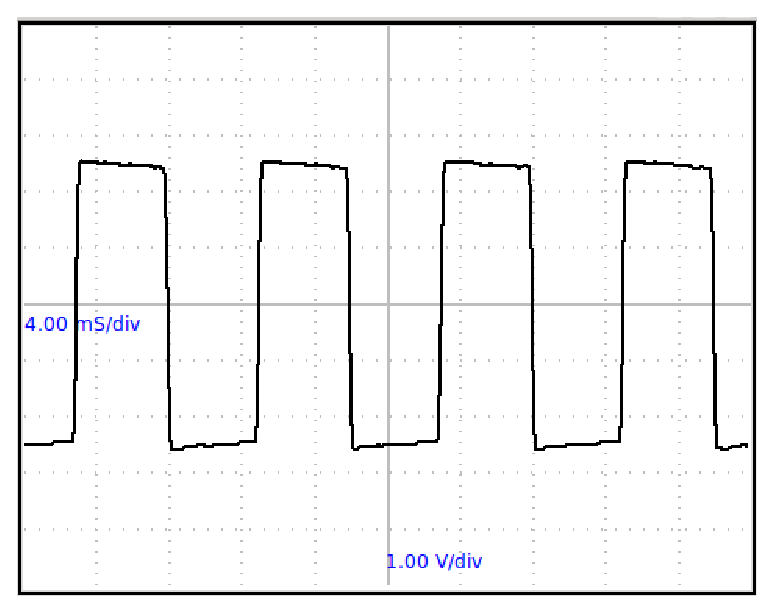
\includegraphics[width=3.3cm]{pics/sqrwave_dcblocked}
\par\end{centering}

\caption{Voltage swinging between 0 and 5 volts (a) Direct connection (b) With
a DC blocking capacitor\label{fig:Square-wave}}
\end{figure}

\begin{itemize}
\item 1~\textmu{}F capacitor, 10~k$\Omega$ resistor
\end{itemize}

\subsection*{Procedure}
\begin{itemize}
\item Connect SQR1 to A0 using the wire.
\item Enter\textit{500} in the Textbox of SQR1 and press Enter key.
\item Adjust the horizontal scale to see several cycles.
\item Insert a 1~\textmu{}F between SQR1 and A0
\item Connect 10~k$\Omega$ from A0 to ground.
\end{itemize}

\subsection*{Observation}

The observed waveforms with and without the series capacitor are shown
in figure\ref{fig:Square-wave}. The voltage is swinging between 0
and 5 volts. After passing through the capacitor the voltage swings
from -2.5 volts to +2.5 volts.


\subsection*{Discussion}

What will you get if subtract a 2.5 from the y-cordinate of every
point of the first graph. That is what the capacitor did. It did not
allow the DC part to pass through.

This original voltage can be considered as a 5V AC superimposed on
a 2.5V DC.

You may need to connect a 10$k\Omega$ resistor from A0 to Ground
to see a waveform swinging between -2.5 to +2.5 volts.

Why the resistor is required?\newpage{}


\section{Resistance of human body}


\subsection*{Objective}

Get some idea about the resistance of the human skin and how it varies.


\subsection*{Equipment}
\begin{itemize}
\item Two pieces of wire.
\end{itemize}

\subsection*{Procedure}
\begin{itemize}
\item Set SQR1 to 500
\item make a connection from SQR1 to A0, through your body
\item Adjust the horizontal scale to see several cycles.
\item Repeat the same by using SINE instead of SQR1.
\end{itemize}

\subsection*{Observation}

\begin{figure}
\begin{centering}
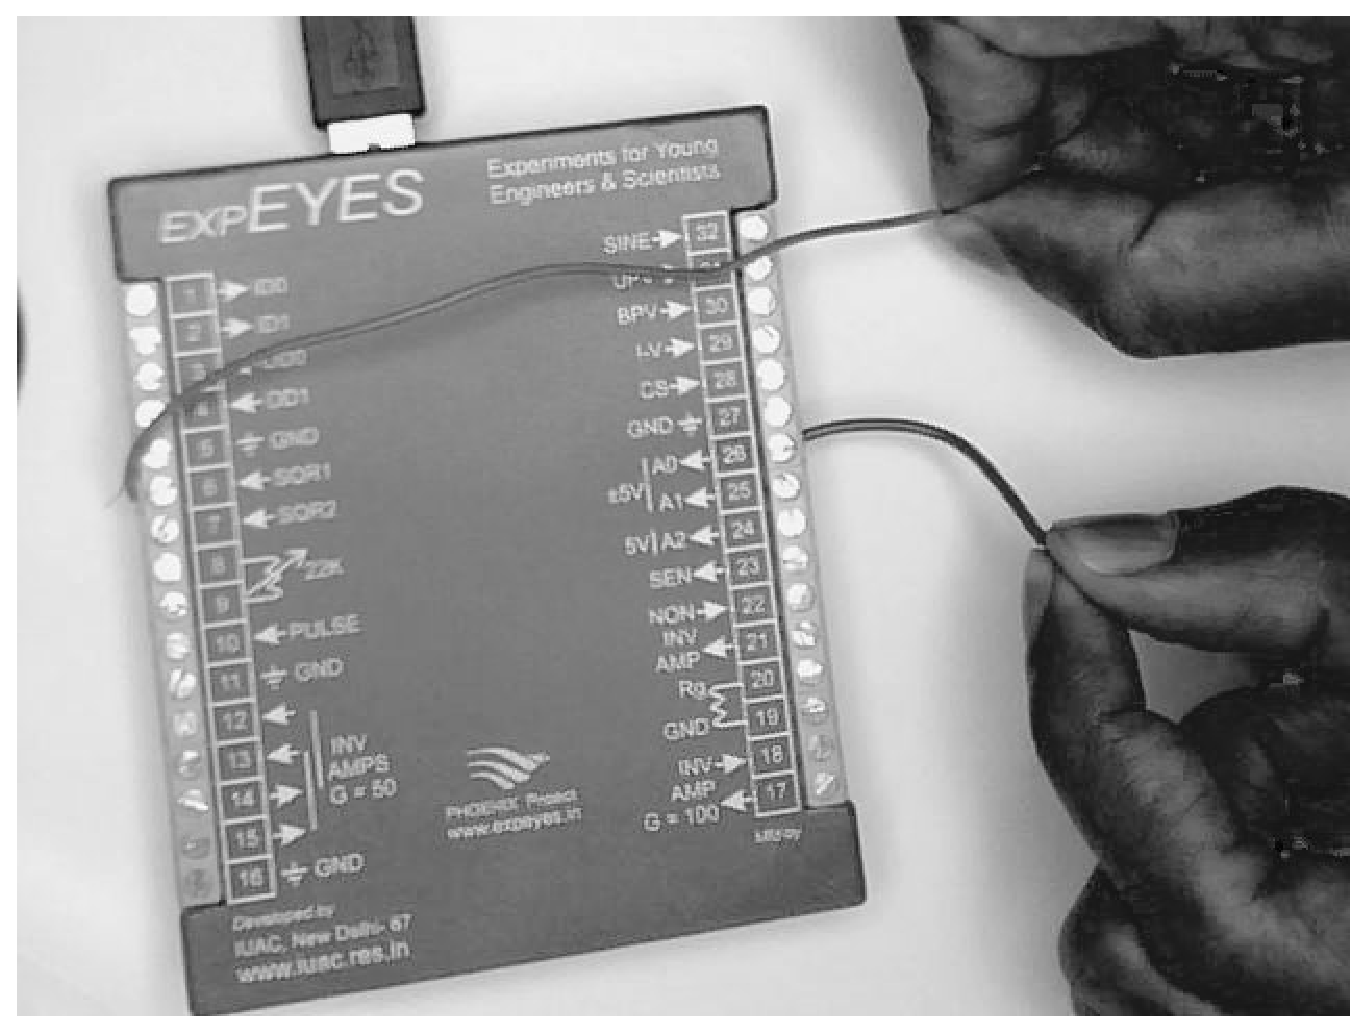
\includegraphics[width=4.1cm]{pics/conduct-hand}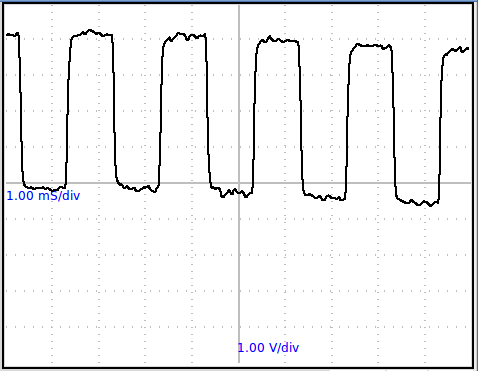
\includegraphics[width=4cm]{pics/sqrwave_hand}
\par\end{centering}

\caption{Voltage after passing through the hand.\label{fig:Square-wave-hand}}
\end{figure}


The observed waveform is shown in figure\ref{fig:Square-wave-hand}.
The wave is not clean and the amplitude is reduced from 5 volts.


\subsection*{Discussion}

Using the method of comparison, try to calculate the resistance of
the portion of the hand between the two wires, you were holding. The
reference resistance is 10$M\Omega$, internally connected from A0
to ground.

\newpage{}


\section{Temperature dependent resistors}


\subsection*{Objective}

Show the dependence of resistance on temperature. Basic concept of
a temperature sensor.


\subsection*{Equipment}
\begin{itemize}
\item Thermistor (NTC)%
\footnote{Negative Temperature Coefficient%
}. Resistance$1k\Omega$ at 25 degree Celsius.
\item Cold water
\item A candle or some other heat source.
\end{itemize}

\subsection*{Procedure}


\includegraphics[height=0.8cm]{schematics/ntc}
\begin{itemize}
\item Connect the Thermistor (NTC) from CS to ground
\item Set CS to 1.0 mA
\item Measure the voltage across the thermistor at different temperatures
\end{itemize}

\subsection*{Observation}

\begin{tabular}{|c|c|c|}
\hline 
Setup & V=IR & $R=\frac{V}{I}$\tabularnewline
\hline 
\hline 
Place in cold water & 1.2 & 1200\tabularnewline
\hline 
Room Temperature & 0.935 & 935\tabularnewline
\hline 
\end{tabular}


\subsection*{Discussion}

Why materials show electrical resistance ?

Why it depends on temperature ?

For metals, R increases with T. But for insulators and semiconductors
it decreases. Why ?

What is the meaning of temperature at molecular level ?

\newpage{}


\section{Light dependent resistors}


\subsection*{Objective}

Learn about LDR. Measure intensity of light and its variation with
distance from the source.


\subsection*{Equipment}
\begin{itemize}
\item A Light Dependent Resistor, LDR
\item 10k$\Omega$ resistor
\item A torch bulb without any reflector.
\end{itemize}

\subsection*{Procedure}


\includegraphics[height=0.8cm]{schematics/ldr}
\begin{itemize}
\item Connect LDR between UPV and A2
\item set UPV to 4 volts.
\item 10~k$\Omega$ resistor from A2 to ground
\item Measure the voltage at A2, with no light on LDR.
\item Measure it by keeping the torch bulb at a distance%
\footnote{Need to be done in a dark room%
}.
\item Change the distance and note down the voltage at A2.
\item Calculate the resistance by camparison as described in section\ref{sec:Measure-resistance-by}
\end{itemize}

\subsection*{Observation}

The resistance vary from 1~k$\Omega$ to around 100~k$\Omega$ depending
on the intensity of light falling on it.


\subsection*{Discussion}

The voltage is proportional to the resistance. The resistance decreases
with intensity of light. If you use a point source of light, the resistance
should increase as the square of the distance.

\newpage{}


\section{Electricity through liquids, DC \& AC}


\subsection*{Objective}

Measure the resistance of liquids. Using both DC and AC voltages.


\subsection*{Equipment}

\begin{figure}
\begin{centering}
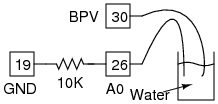
\includegraphics[width=3.9cm]{schematics/water}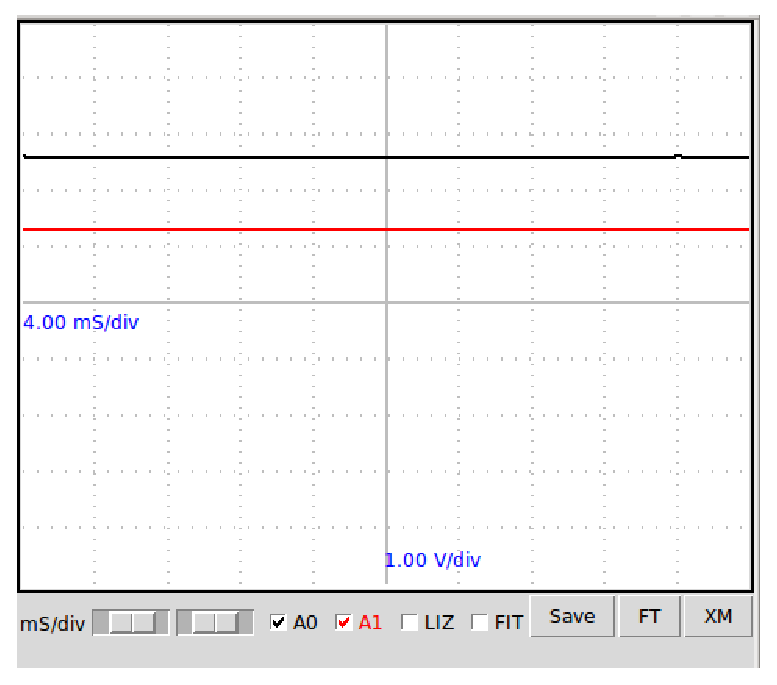
\includegraphics[width=3.6cm]{pics/DCthrough_water}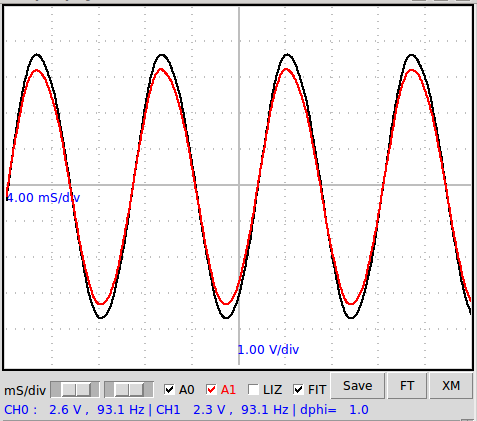
\includegraphics[width=3.6cm]{pics/ACthrough_water}
\par\end{centering}

\caption{(a)Experimrntal setup. (b)Total DC voltage and voltage across the
1k$\Omega$ resistor. (c) Total AC voltage and voltage across 1k$\Omega$
resistor.\label{fig:Current through water}}
\end{figure}

\begin{itemize}
\item A 100 ml beaker
\item Common salt
\item 10k resistor
\end{itemize}

\subsection*{Procedure}
\begin{itemize}
\item Take some tap water in the beaker
\item Connect a wire to BPV and place other end in water
\item Another wire from A0 to water
\item Connect 10k resistor from A0 to ground.
\item Set 2.8 volts on BPV and watch the value of A0%
\footnote{If the voltage is too low use a higher resistance than 10k, otherwise
use a lower one.%
}
\item Try changing BPV from +2.8V to -2.8V and watch the horizontal trace.
\item Repeat the experiment using AC from SINE instead of DC from BPV
\item Calculate the resistance as explained in section\ref{sec:Measure-resistance-by}
\end{itemize}

\subsection*{Observation}

\begin{tabular}{|c|c|c|c|c|c|}
\hline 
 & $V_{total}$ & $V_{10k\Omega}$ & $V_{liq}$ & $I=\frac{V_{10k\Omega}}{1000}$ & $R_{liq}=\frac{V_{liq}}{I}$\tabularnewline
\hline 
\hline 
AC & 2.6 & 2.3 & 0.3 & .23 mA & 1.3 k$\Omega$\tabularnewline
\hline 
DC & 2.6 & 1.3 & 1.3 & .13 mA & 10 k$\Omega$\tabularnewline
\hline 
\end{tabular}

Observed values are shown in the table%
\footnote{The values you may get could be very different depending on the ion
concentration and presence of impurities in the water used.%
}. The DC and AC resistances seems to be very different. However, when
you change the polarity of BPV, the voltage across the resistor stays
around the AC value for a while and then goes down. This indicates
that the resistance of the liquid increases with time, may be due
to some bubble formation.


\subsection*{Discussion}

Why the behavior is different for AC and DC ?

What are the charge carriers responsible for the flow of electricity
through solutions ?

Is there any chemical reaction taking place ?

Try adding some common salt and repeat the measurements.

\newpage{}


\section{Transient Response of RC circuits\label{sec:Capacitor-charging-&}}


\subsection*{Objective}

In section\ref{sec:DC-&-AC}, we have seen that a capacitor blocks
DC but allows AC to pass through. In this experiment, we will explore
the nature of current and voltage when a voltage step is applied.
By measuring the voltage across the capacitor as a function of time,
we can calculate the value of the capacitance.


\subsection*{Theory}

Voltage across a capacitor while charging through a resistor
\[
V(t)=V_{0}\left(1-e^{-\frac{t}{RC}}\right)
\]


\begin{flushleft}
Voltage across a capacitor while discharging through a resistor
\[
V(t)=V_{0}e^{-\frac{t}{RC}}
\]

\par\end{flushleft}


\subsection*{Equipment}

\begin{figure}
\begin{centering}
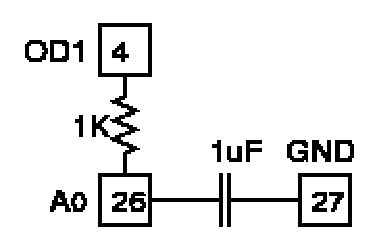
\includegraphics[width=3.2cm]{schematics/rc-tran}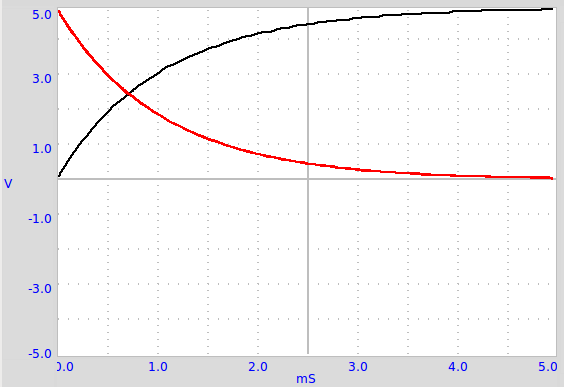
\includegraphics[width=3.8cm]{pics/CR-transient-screen}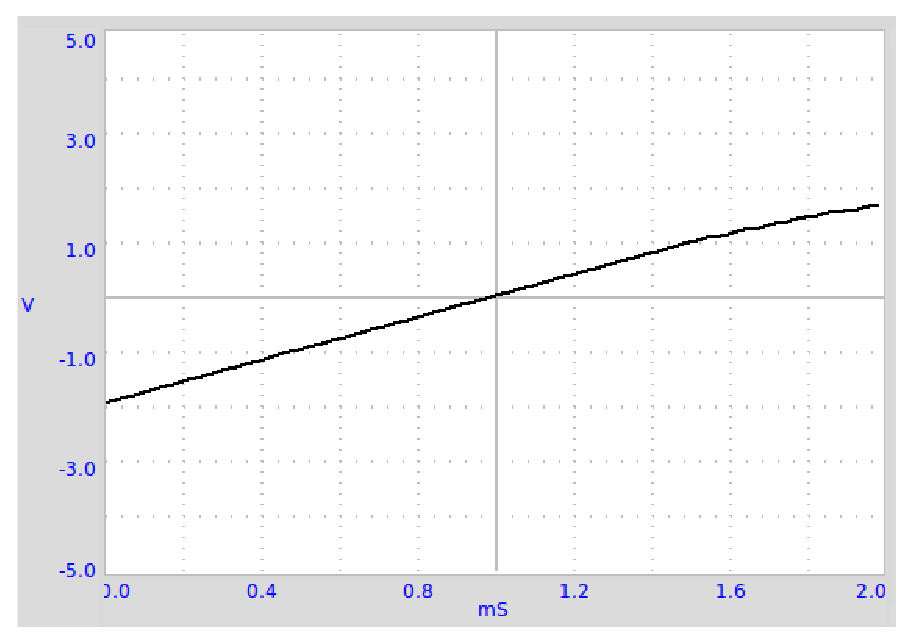
\includegraphics[width=3.8cm]{pics/capacitor_linear}
\par\end{centering}

\caption{Transient response of RC circuit. The third one is the charging of
a capacitor through a constant current source.\label{fig:Capacitor-screenshot}}
\end{figure}

\begin{itemize}
\item A$1\mu F$ capacitor and a$1k\Omega$ resistor.
\end{itemize}

\subsection*{Procedure}
\begin{itemize}
\item Connect the capacitor from A0 to Ground.
\item Connect the resistor from A0 to OD1.
\item Right click on the Panel and select\textit{\menuitem{RC Circuit}}
from the pop-up menu
\item Click on\textit{\emph{\buttonlabel{0->5V STEP}}} and\textit{\emph{\buttonlabel{5->0VSTEP}}}
Buttons to plot the graphs
\item Adjust the horizontal scale, if required, and repeat.
\item FIT the curve to extract the time constant RC.
\end{itemize}

\subsection*{Observation}

Applying a 0 to 5V step makes the voltage across the capacitor to
rise exponentially as shown in the figure\ref{fig:Capacitor-screenshot}.
By fitting the graph we can extract the RC time constant and find
the values of capacitance from it.

This experiment can be extended to masure die-electric constant of
materials by making capacitors using them. To get the graph shown
in\ref{fig:Capacitor-screenshot}(c), connect R from CS to A0, C from
OD1 to A0, set CS to 1mA and click on\textit{5->0V.}


\subsection*{Discussion}

Why the graph is Exponential ?

A capacitor is made of two parallel metal plates separated by a thin
layer of dielectric material. We have connected one plate (call it
plate A) to ground and another plate (call it B) to OD1 via a resistor.
Connection to A0 is for monitoring the voltage. Initially both plates
are at zero volts. By clicking on\textit{0->5V} ,we take OD1 to 5
volts. A current will start flowing through the resistor to plate
B, due to the potential difference created. This current (flow of
charge) will result in an accumulation a charge on plate B. The voltage
at B will be given by$V=Q/C$, where Q is called the capacitance.
As more and more charge arrives, voltage at B also will increase.
But, as per Ohm's law the current through the resistor is decided
by the voltage difference across it. That mean the current will gradually
decrease and reach zero when the voltage at plate B becomes 5 volts.
The time for this is decided by the product RC, and is given by

\[
V(t)=V_{0}\left(1-e^{-\frac{t}{RC}}\right)
\]


The product RC is called the time constant of the circuit.\textit{}%
\footnote{\textit{http://hyperphysics.phy-astr.gsu.edu/hbase/electric/capchg.html}%
}

\newpage{}


\section{Transient Response of RL circuits}


\subsection*{Objective}

Explore the nature of current and voltage when a voltage step is applied
to resistor and inductor in series. By measuring the voltage across
the inductor as a function of time, we can calculate its value.


\subsection*{Theory}

In an RL circuit$V=IR+L\frac{dI}{dt}$ . Solving this will give$I=I_{0}e^{-\frac{R}{L}t}$
. The coefficient of the exponential term R/L can be extracted from
the graph of voltage across the inductor. The resistance of the inductor
coil should be included in the calculations,$R=R_{ext}+R_{L}$.%
\footnote{http://nptel.iitm.ac.in/courses/Webcourse-contents/IIT-KANPUR/esc102/node14.html%
}


\subsection*{Equipment}

\begin{figure}
\begin{centering}
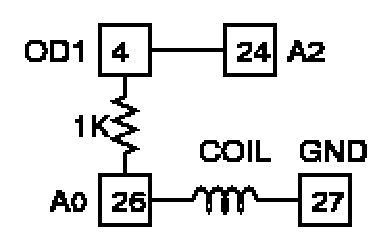
\includegraphics[width=3.2cm]{schematics/rl-tran}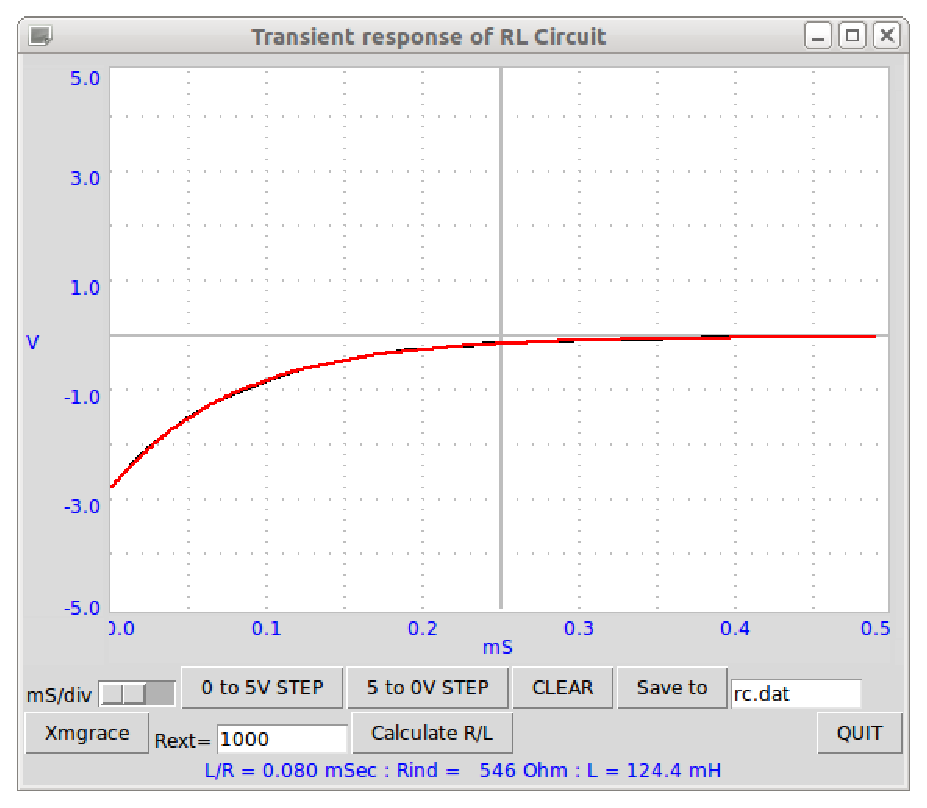
\includegraphics[width=4cm]{pics/LR-downstep}
\par\end{centering}

\caption{LR circuit. Voltage across the inductor after a 5 to 0V step.\label{fig:LR-circuit.-Voltage}}
\end{figure}

\begin{itemize}
\item $1k\Omega$ resistor.
\item 3000 turns coil, 1000 turns coil \& ferrite core
\end{itemize}

\subsection*{Procedure}
\begin{itemize}
\item Connect the 3000 Turns coil from A0 to Ground.
\item Connect the resistor from A0 to OD1.
\item Connect a wire from OD1 to A2 (for accurate measurement of total voltage)
\item Right click on the Panel and select\textit{\menuitem{RL Circuit}}
from the pop-up menu
\item Click on\foreignlanguage{french}{\textit{\emph{\buttonlabel{0->5V STEP}}}}
and\foreignlanguage{french}{\textit{\emph{\buttonlabel{5->0V STEP}}}}
Buttons to plot the graphs
\item Adjust the horizontal scale, if required, and repeat.
\item Calculate the value of inductance
\item Repeat by inserting core. Repeat with other coils.
\end{itemize}

\subsection*{Observation}

The Voltage across the inductor just after a 5V to 0V step is shown
in figure\ref{fig:LR-circuit.-Voltage}. The exponential curve is
fitted to extract the L/R value. The resistance of the coil is measured
by comparing it with the known external resistance under DC conditions.
The inductances measured are tabulated below.

\begin{tabular}{|c|c|c|}
\hline 
Coil & Inductance (mH) & Resistance ($\Omega$)\tabularnewline
\hline 
\hline 
3000 Turns coil & 126 & 565\tabularnewline
\hline 
1000 T & 4.7 & 42\tabularnewline
\hline 
1000T /ferrite & 25 & 42\tabularnewline
\hline 
\end{tabular}


\subsection*{Discussion}

The applied voltages are above zero, but the graph went to negative
voltages. Why ?

What was the current before doing the 5->0 step ? What is back EMF
?

\newpage{}


\section{Transient response of LCR circuits\label{sec:Step-Response-ofRLC}}


\subsection*{Objective}

The response of RL and RC circuits were done in the previous sections.
Now we will explore the oscillatory nature by connecting L and C in
series.


\subsection*{Theory}

Resonant frequency of series LC circuit =$\omega_{0}=\frac{1}{2\pi\sqrt{LC}}$,
Damping factor =$\frac{R}{2}\sqrt{\frac{C}{L}}$, equal to 1 for critical
damping.%
\footnote{http://en.wikiversity.org/wiki/RLC\_circuit%
}


\subsection*{Equipment}

\begin{figure}
\begin{centering}
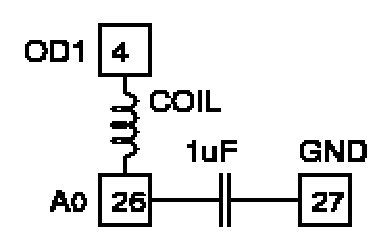
\includegraphics[width=3cm]{schematics/lc-tran}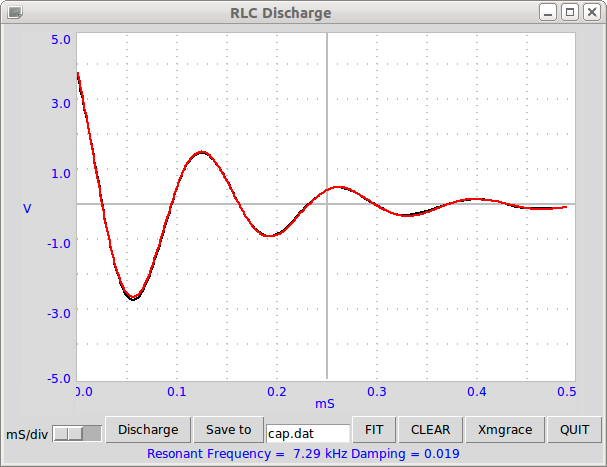
\includegraphics[width=3.5cm]{pics/LCRdischarge}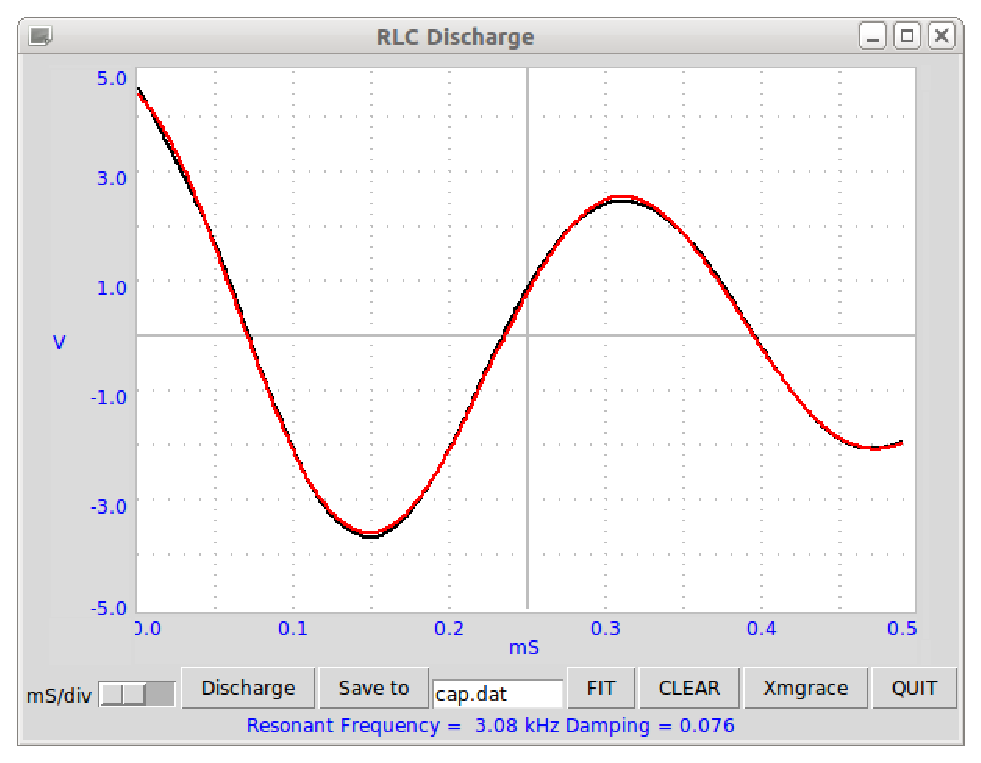
\includegraphics[width=3.5cm]{pics/LCRdischarge_ferrite}
\par\end{centering}

\caption{Transient response of LCR circuit. (a)~Setup (b)~Result with air
core inductor. (c)~With ferrite core\label{fig:LCR-response-setup}}
\end{figure}

\begin{itemize}
\item 0.1uF capacitor
\item 3000 \& 1000 Turns coil
\item Ferrite core
\end{itemize}

\subsection*{Procedure}
\begin{itemize}
\item Connect Coil from OD1 to A0
\item Capacitor from A0 to ground
\item Right-click on Panel and select\textit{\menuitem{RLC Discharge}}
from the menu.
\item Click on Discharge. Adjust x-axis and repeat if required.
\item FIT the graph to find the resonant frequency \& Damping.
\item Repeat the experiment with ferrite core inserted
\item Repeat with a 1$k\Omega$ resistor in series.
\end{itemize}

\subsection*{Observation}

\begin{figure}
\begin{centering}
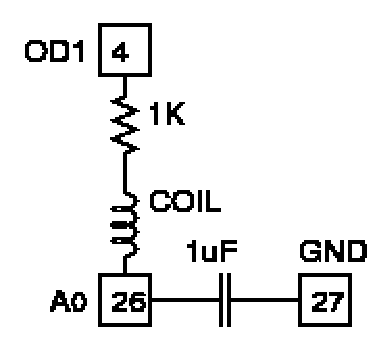
\includegraphics[width=3cm]{schematics/rlc-tran}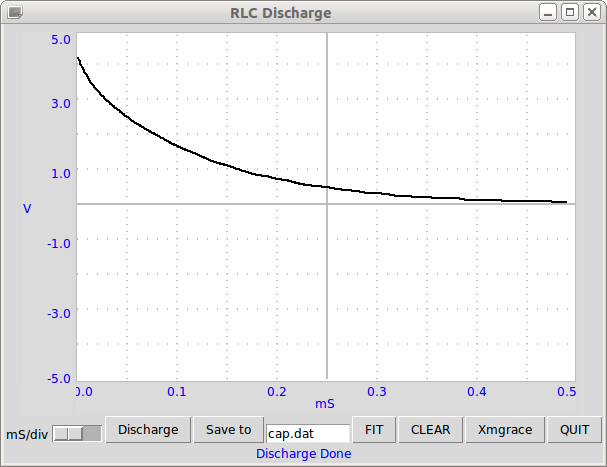
\includegraphics[width=4cm]{pics/LCRdischarge_1k}
\par\end{centering}

\caption{LCR with a 1k series resistor providing damping.\label{fig:LCR-response-screen}}
\end{figure}


Measurements have been done using the 1000 Turns coil, with and without
ferrite core, and the 3000 Turn coil. The results are tabulated below.
The capacitance and inductance were measured by an LCR meter.

\begin{tabular}{|c|c|c|c|}
\hline 
C$\mu F$ & L mH & $f=\frac{1}{2\pi}\sqrt{\frac{1}{LC}}$ & $f_{measured}(Hz)$\tabularnewline
\hline 
\hline 
.097 & 3.57 & 8552 & 8430\tabularnewline
\hline 
.097 & 23.2 & 3354 & 3400\tabularnewline
\hline 
.097 & 125 & 1445 & 1400\tabularnewline
\hline 
\end{tabular}


\subsection*{Discussion}

The under damped waveform require a resistance,$R=\sqrt{\frac{4L}{C}}=\sqrt{\frac{4\times23.2e-3}{.097e-6}}=963$
to make it critically damped. Result with a 1k$\Omega$ series resistor
is shown in figure .

Why the amplitude went up after inserting the ferrite core ?

\newpage{}


\section{Capacitor in AC circuits\label{sec:Capacitor-in-AC}}


\subsection*{Objective}

Explore the effect of a series capacitor in AC circuits, under steady
state conditions.


\subsection*{Theory}

Impedance of a Capacitor$X_{c}=\frac{1}{2\pi fC}$ , where$f$ is
the frequency in Hertz and$C$ is the capacitance in Farads. Remember
the working of a capacitor explained in section\ref{sec:Capacitor-charging-&}.

\begin{figure}
\begin{centering}
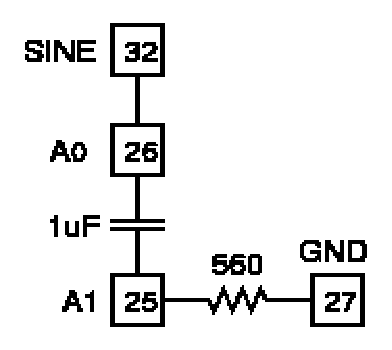
\includegraphics[width=3cm]{schematics/rc-steadystate}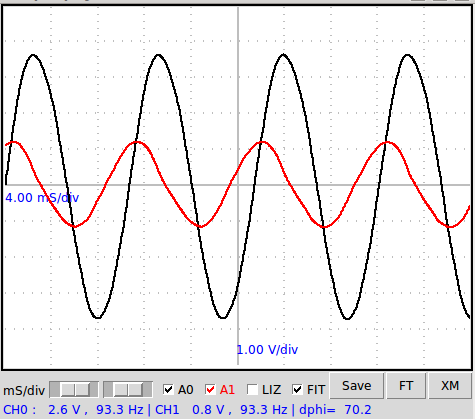
\includegraphics[width=4cm]{pics/CRphaseshift-1uf560}
\par\end{centering}

\caption{Screenshot showing the total voltage across the RC circuit and the
voltage across the capacitor. C=1 uF and R = 560$\Omega$.\label{fig:CRcircuit_voltages}}
\end{figure}



\subsection*{Equipment}
\begin{itemize}
\item 1 uF capacitor
\item 560$\Omega$ resistor
\item A voltmeter, if you want to measure the voltage across the elements
not directly connected to ground.
\end{itemize}

\subsection*{Procedure}
\begin{itemize}
\item Connect a wire from SINE to A0
\item Connect the capacitor from A0 to A1
\item Connect resistor from A1 to Ground.
\item Enable A1 also. Adjust the horizontal scale to view more than 4 cycles.
\item Enable 'FIT' to show RMS voltage, Frequency etc.
\end{itemize}

\subsection*{Observation}

The input waveform and the voltage across the resistor\ref{fig:CRcircuit_voltages}.
The voltage across the capacitor is calculated using Ohm's law, you
can also measure it with a volt meter.

The sum of the two voltages looks like more than the total applied
voltage.

Are we violating Ohm's Law ?

What mistake we are making while adding the voltages ?

\begin{tabular}{|c|c|c|c|c|}
\hline 
$V_{Tot}$ & $V_{Res}$ & $I=\frac{V_{res}}{R}$ & $V_{cap}=IX_{c}$ & $V_{R}+V_{c}$\tabularnewline
\hline 
\hline 
2.6 & .8 & 0.0014 & 2.4 & 3.2\tabularnewline
\hline 
\end{tabular}

$X_{c}=\frac{1}{2\pi fC}=\frac{1}{2\pi\times93.6\times1e-6}=1712$

$V_{c}=IX_{c}=1712\times0.0014$


\subsection*{Discussion}

We need to account for the phase shift introduced by the capacitor%
\footnote{http://www.play-hookey.com/ac\_theory/ac\_rc\_series.html%
}. Refer to the next section.

\newpage{}


\section{AC phase shift in RC circuits}


\subsection*{Objective}

Measure the AC voltage phase shift across the capacitor in an RC circuit.


\subsection*{Theory}

In an RC circuit, the phase shift across the inductor is given by
the equation$\triangle\Phi=\arctan\left(\frac{X_{c}}{R}\right)$,
where R is the resistance and$X_{c}$ is the capacitive reactance.

\begin{figure}
\begin{centering}
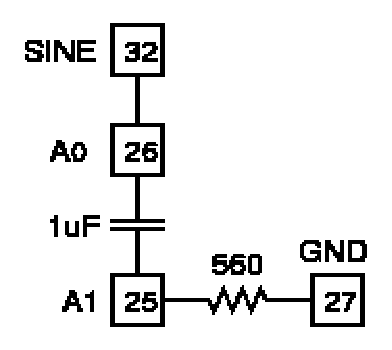
\includegraphics[width=3cm]{schematics/rc-steadystate}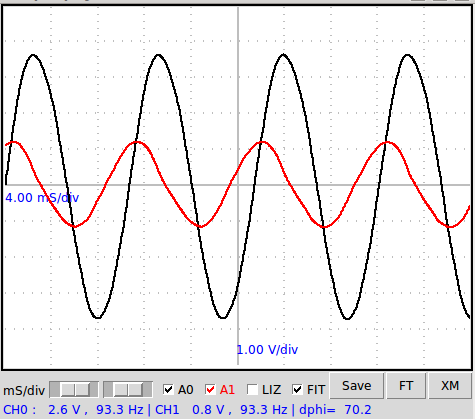
\includegraphics[width=4cm]{pics/CRphaseshift-1uf560}
\par\end{centering}

\caption{Screenshot showing phase shifts for R=560$\Omega$ and C = 1$\mu F$.\label{fig:RC phaseshift}}
\end{figure}



\subsection*{Equipment}
\begin{itemize}
\item 1 uF capacitor
\item 560$\Omega$ resistor (Try other values also)
\end{itemize}

\subsection*{Procedure}
\begin{itemize}
\item Connect a wire from SINE to A0
\item Connect the capacitor between A0 and A1
\item Connect Resistor from A1 to Ground.
\item Enable A1 also. Adjust the horizontal scale to view more than 4 cycles.
\item Enable 'FIT' to show RMS voltage, Frequency and Phase difference.
\end{itemize}

\subsection*{Observation}

The measured phase shifts are tabulated below. The connections and
the voltage waveforms are shown in figure\ref{fig:RC phaseshift}.

\begin{tabular}{|c|c|c|c|c|}
\hline 
C(uF) & R(k$\Omega$) & Freq (Hz) & $\bigtriangleup\Phi$ & $\arctan\left(\frac{X_{c}}{X_{R}}\right)$\tabularnewline
\hline 
\hline 
1 & 560 & 93 & 71.3 & 71.9\tabularnewline
\hline 
\end{tabular}

where$X_{c}=\frac{1}{2\pi fC}$ is the impedance of the capacitor,
Frequency is 93Hz.$X_{R}$ is the resistance.

Current through a capacitor leads the voltage across it by$90^{0}$.
Why ?


\subsection*{Discussion}

Why the phase of the voltage advances ? Assume we have connected the
AC to plate A and at an instance$t=t_{0}$ the input voltage is at
zero volts. We can see that the slope of the curve is maximum there,
ie. the rate of change of voltage is maximum. The capacitor gets charged
very fast at this point. The plate B also gathers the same charge
as plate A , that is how a capacitor works. The current to plate B
is flowing from ground through the resistor and we are measuring the
IR drop across the resistor, it will be already positive when plate
A is at zero. This results in the phase advance.

\newpage{}


\section{AC phase shift in RL circuits\label{sec:Inductor-in-AC}}


\subsection*{Objective}

Measure the AC voltage phase shift in an RL circuit.


\subsection*{Theory}

Impedance of an Inductor$X_{L}=2\pi fL$ , where$f$ is the frequency
in Hertz and L is the inductance in Henry. In an LC circuit, the phase
lag across the inductor is given by the equation$\triangle\Phi=\arctan\left(\frac{X_{L}}{R}\right)$,
where R is the resistance in Ohms.


\subsection*{Equipment}

\begin{figure}
\begin{centering}
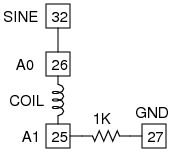
\includegraphics[width=3cm]{schematics/rl-steadystate}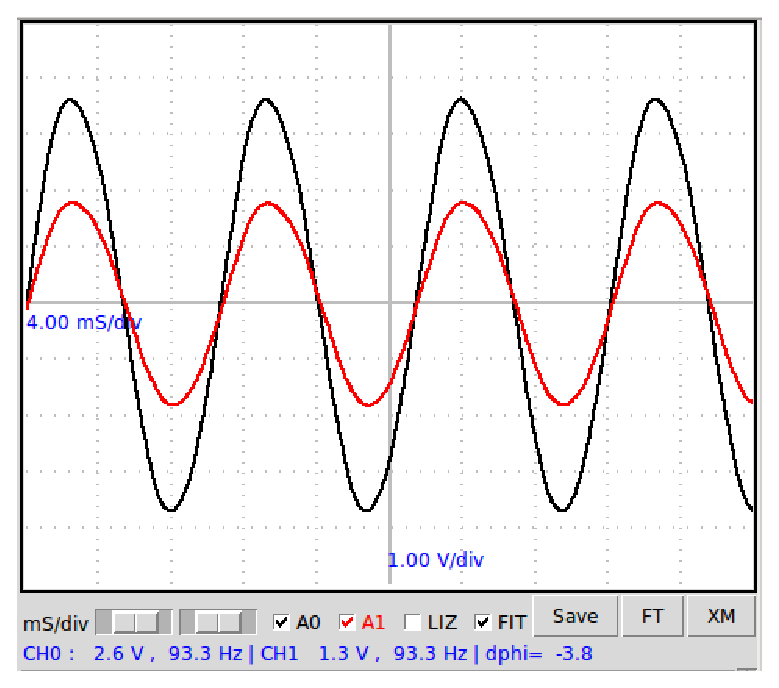
\includegraphics[width=4cm]{pics/LRphaseshift-125mH-125ohm}
\par\end{centering}

\caption{Sine wave to LR circuit. Phase shift across inductor\label{fig:LR  phaseshift-screen}}
\end{figure}

\begin{itemize}
\item Inductor, use the solenoid coils supplied.
\item 560$\Omega$ and 1$k\Omega$ resistors
\end{itemize}

\subsection*{Procedure}
\begin{itemize}
\item Connect a wire from SINE to A0
\item Connect the Inductor between A0 and A1
\item Connect the 1k$\Omega$ resistor from A1 to Ground.
\item Enable A1 also. Adjust the horizontal scale to view more than 4 cycles.
\item Enable 'FIT' to show RMS voltage, Frequency and Phase difference.
\end{itemize}

\subsection*{Observation}

The measured phase shifts are shown below. Waveforms for the 125 mH
inductor is shown in figure\ref{fig:LR  phaseshift-screen}. The resistance
of the inductor also should be included while calculating the phase
shift.

\begin{tabular}{|c|c|c|c|}
\hline 
L(mH) & $R=R_{coil}+R_{ext}$($\Omega$) & $\bigtriangleup\Phi=\arctan\left(\frac{X_{L}}{X_{R}}\right)$ & $\bigtriangleup\Phi_{measured}$\tabularnewline
\hline 
\hline 
125 & 565 + 560 & 3.71 & -3.8\tabularnewline
\hline 
25 & 42 + 560 & 1.39 & -1.4\tabularnewline
\hline 
\end{tabular}

Current through an inductor lags by$90^{0}$%
\footnote{http://www.play-hookey.com/ac\_theory/ac\_inductors.html%
}.


\subsection*{Discussion}

If you do not know the value of an inductor, you can use this experiment
to determine it from the phase shift observed with a known resistor
value.

\newpage{}


\section{Ferromagnetic material inside inductor}


\subsection*{Objective}

Observe the effect of ferromagnetic materials inside a solenoid coil
inductor.


\subsection*{Theory}

Self Inductance of a solenoid is given by$L=\frac{\mu N^{2}A}{l}$
, where N is the number of turns, A is the cross sectional area,$\mu$
is the permeability of the surrounding media and$l$ is the length.

\begin{figure}
\begin{centering}
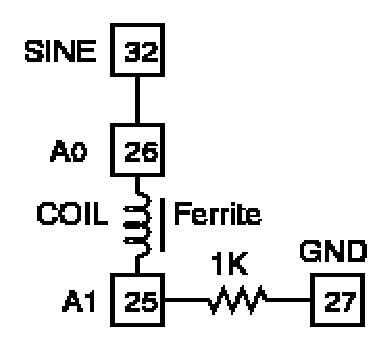
\includegraphics[width=3cm]{schematics/rl-steadystate-ferrite}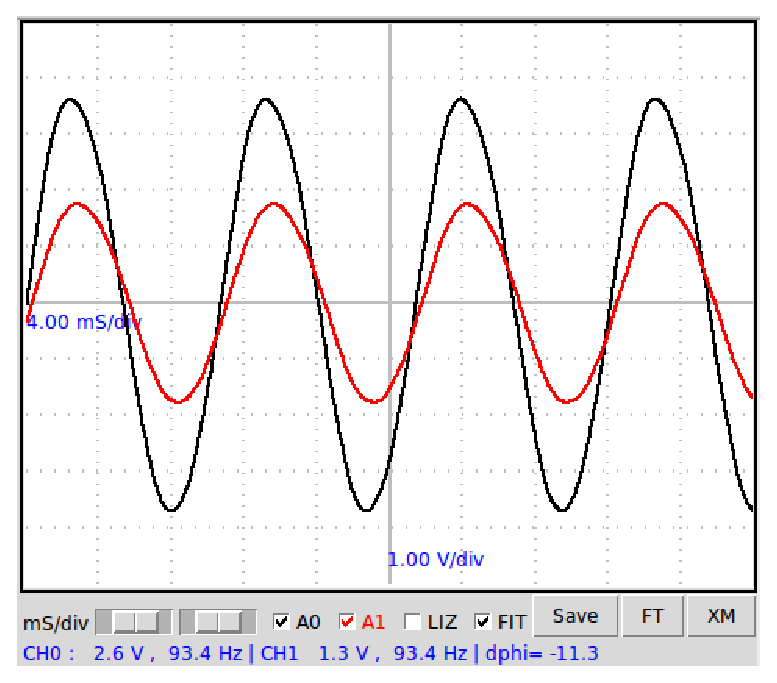
\includegraphics[width=4cm]{pics/LRphaseshift_ferrite}
\par\end{centering}

\caption{LR circuit. Effect of Ferrite core.\label{fig:Ferrite_LR-screen}}
\end{figure}



\subsection*{Equipment}
\begin{itemize}
\item 1000 turns coil
\item 1$k\Omega$ resistor (You can use other values also)
\end{itemize}

\subsection*{Procedure}
\begin{itemize}
\item Connect as explained in\ref{sec:Inductor-in-AC}
\item Insert an ion rod into the coil and observe the changes
\item Repeat with the 3000 turns coil.
\end{itemize}

\subsection*{Observation}

The phase shift increased from 3.7 to 11.6 by inserting the ferrite
core.


\subsection*{Discussion}

The phase shift went from 3.7 to 11.6 degrees, around 3 times increase
in the Inductance. However, in this case it will be wrong to assume
that the permeability of the core is 3 Why ? (look at the geometry)

\newpage{}


\section{RC Integration \& Differentiation}


\subsection*{Objective}

Integrate and differentiate a squarewave using and RC circuit.


\subsection*{Theory}

\begin{figure}
\begin{centering}
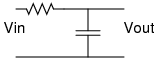
\includegraphics[width=4cm]{pics/RCinteg}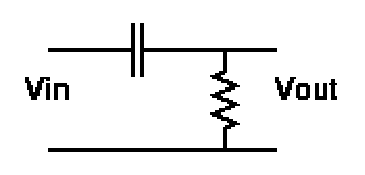
\includegraphics[width=4cm]{pics/RCdiff}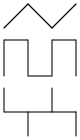
\includegraphics[width=1.6cm]{pics/triwave_diff}
\par\end{centering}

\caption{(a)RC Intergrator (b)RC Differentiator (c) Square wave, integrated
and differentiated.\label{fig:RC-Integ-diff}}
\end{figure}


For the circuit shown in figure\ref{fig:RC-Integ-diff}(a)

\[
V_{out}=\frac{1}{RC}\int V_{in}dt
\]


and for the one in figure\ref{fig:RC-Integ-diff}(b)
\[
V_{out}=RC\frac{dV_{in}}{dt}
\]


Figure\ref{fig:RC-Integ-diff}(c) shows a square wave, with it's integrated
and differentiated outputs. It is easy to understand as the triagular
wave differentiated twice. The constant positive slope of triangular
wave gives the positive horizontal part of the square wave. Differentiating
the square wave gives spikes at the rising and falling edges. These
are ideal cases.


\subsection*{Equipment}
\begin{itemize}
\item 1uF capacitor
\item 1$k\Omega$ resistor
\end{itemize}

\subsection*{Procedure}

\includegraphics[height=0.8cm]{schematics/rc-integ}~~~\includegraphics[height=0.8cm]{schematics/rc-diff}
\begin{itemize}
\item Connect a wire from SQR1 to A0
\item Connect R from SQR1 to A1
\item Connect C from A1 to Ground.
\item Enable A1. Adjust the horizontal scale to view more than 4 cycles.
\item Set SQR1 to 20Hz, 100Hz and 1kHz and view the waveforms.
\item Interchange the positions of R and C to watch differentiation.
\item Click on the Button\buttonlabel{FT} to view a Fourier Transform.
\end{itemize}

\subsection*{Observation}

\begin{figure}
\begin{centering}
\includegraphics[width=3.6cm]{pics/squarewave_interg20hz}\includegraphics[width=3.6cm]{pics/squarewave_interg1khz}\includegraphics[width=3.6cm]{pics/squarewave_diff20hz}
\par\end{centering}

\caption{(a) Integration at 20Hz (b)Integration at 1kHz (c) Differentiation
at 20Hz. For all cases R=1k$\Omega$ and C=1uF\label{fig:Effect-of-RCon squarewave}.}
\end{figure}


Integration observed at 20Hz and 1kHz are shown in figure\ref{fig:Effect-of-RCon squarewave},
using an RC of 1 milliseconds. At 20Hz, the squarewave passes through
the cpacitor with a small distortion.


\subsection*{Discussion}

When the time period becomes comparable with the RC value, the waveform
becomes triangular. The differentiation can only be shown at lower
frequency since capturing the narrow spike require a fast oscilloscope.

\newpage{}


\section{Fourier Analysis\label{sec:Fourier-Transform-**}}


\subsection*{Objective}

Learn about Fourier Transform of a signal. Time and Frequency domain
representations.


\subsection*{Equipment}
\begin{itemize}
\item A piece of wire.
\end{itemize}

\subsection*{Procedure}
\begin{itemize}
\item Connect SINE to A0
\item Adjust the horizontal scale to view several cycles.
\item Click on FT to do a Fourier tarnsform
\end{itemize}

\subsection*{Observation}
\begin{itemize}
\item The sinewave and it's Fourier transform are shown in figure\ref{fig:Sine-wave-and}.
\end{itemize}
\begin{figure}
\begin{centering}
\includegraphics[width=6cm]{pics/sinewave}\includegraphics[width=5cm]{pics/sine90hz-fft}
\par\end{centering}

\caption{(a)Sine wave. (b) Frequency spectrum by Fourier transform.\label{fig:Sine-wave-and}}
\end{figure}



\subsection*{Discussion}

The original display was showing the amplitude as a function of time,
and therefore is called the time domain representation of the signal.
In the Fourier transform plot, frequency is on the x-axis and the
y-axis shows the relative strength of the frequency components of
the signal. This is called the frequency domain representation of
the signal.%
\footnote{http://en.wikipedia.org/wiki/Fourier\_transform%
}In this case there is only one dominant peak. The small peak at three
times the fundamental frequency is a measure of distortion of our
sine wave.

\newpage{}


\section{Harmonics of a square wave}


\subsection*{Objective}

Explore the harmonic content of a square wave using Fourier Transform
.


\subsection*{Equipment}
\begin{itemize}
\item A piece of wire.
\end{itemize}

\subsection*{Procedure}
\begin{itemize}
\item Connect terminal 6 (SQR1) to 26 (A0)
\item Enter 100 on the text field near SQR1 and press Enter key.
\item Enable the Yellow Checkbox A0 on the right side window.
\item Adjust the horizontal scale to 10 milliseconds per division.
\item Press A0-FT
\end{itemize}

\subsection*{Observation}

\begin{figure}
\begin{centering}
\includegraphics[width=5.5cm]{pics/sqr1000Hz}\includegraphics[width=5.5cm]{pics/sqr1000Hz-fft}
\par\end{centering}

\caption{Squarewave and it's Fourier transform\label{fig:Squarewave-and-it's}}
\end{figure}

\begin{itemize}
\item A new window opens displaying a trace as shown in figure .
\end{itemize}

\subsection*{Discussion}

Fourier series decomposes any periodic function or periodic signal
into the sum of a set of simple oscillating functions, namely sines
and cosines. A square wave function can be represented as$f(\theta)=sin(\theta)+\frac{sin(3\theta)}{3}+\frac{sin(5\theta)}{5}+\cdots$.
In the Fourier transform of a square wave of frequency$f$ , there
will be a$3f$ component (having an amplitude of one third of$f$
),$5f$ component (amplitude one fifth) etc. as shown in the figure

\newpage{}


\chapter{Electricity \& Magnetism}

Electromagnetic induction is demonstrated using a moving magnet and
a coil powered by an AC voltage. Working of transformer is demonstrated
using two coils. A simple AC generator, capable of generating multi-phase
output, is made using a rotating magnet.


\section{Electromagnetic induction}


\subsection*{Objective}

Explore the voltage induced across a coil by a changing magnetic field.


\subsection*{Equipment}

\begin{figure}
\begin{centering}
\includegraphics[width=5.8cm]{pics/EMinduction-photo}\includegraphics[width=4.9cm]{pics/em_induction}
\par\end{centering}

\caption{Voltage induced on a coil by a moving magnet.\label{fig:EM Induction}}
\end{figure}

\begin{itemize}
\item Small cylindrical magnets.
\item 3000 Tunrns coil and a paper tube to guide the magnet.
\end{itemize}

\subsection*{Procedure}
\begin{itemize}
\item Connect the coil from A0 to Ground.
\item From Panel right-click and open\menuitem{EM Induction}
\item Click on\buttonlabel{Start Scanning}. A horizontal trace should appear
\item Drop the magnet through the coil until a trace is caught.
\item Repeat the process by changing the parameters like magnet strength,
speed etc.
\end{itemize}

\subsection*{Observation}

The result is shown in figure\ref{fig:EM Induction}. The amplitude
inceases with the speed of the magnet. From the graph, we can find
the time taken by the magnet to travel through the coil.


\subsection*{Discussion}

The second peak is bigger than the first peak. Why ? Where will be
the magnet at the zero crossing of the induced voltage?

Drop the magnet from different heights and plot the voltage vs square
root of the height.

\newpage{}


\section{A simple AC generator\label{sec:A-simple-AC}}


\subsection*{Objective}

Measure the frequency and amplitude of the voltage induced across
a solenoid coil by a rotating magnet. Gain some understanding about
the AC generators by looking at the output and the drawbacks of the
setup.


\subsection*{Equipment}

\begin{figure}
\begin{centering}
\includegraphics[width=3cm]{schematics/ac-gen}\includegraphics[width=4cm]{pics/ACgen-output-30pct}
\par\end{centering}

\caption{Voltage output of the AC generator with different speeds of rotation
of the magnet\label{fig:AC generator output}.}
\end{figure}

\begin{itemize}
\item A magnet , D = 10 mm, L = 10 mm
\item DC motor
\item 3000 Turns coil
\end{itemize}

\subsection*{Procedure}
\begin{itemize}
\item Connect the DC motor to PULSE (T10), mount the magnet horizontally.
\item Connect the coil from A0 to ground
\item Hold the coil perpendicular to the axis of rotation of the motor,
close to the magnet. Be careful not to touch it.
\item Set PULSE to 10 (\% duty cycle)
\item Measure the frequency \& amplitude by enabling FIT.
\item Repeat by changing PULSE to 20 , 30 and 40 (NOT beyond that)
\end{itemize}

\subsection*{Observation}

The voltage output is shown in figure\ref{fig:AC generator output}.
The speed of the motor is nearly proportional to the duty cycle (from
20\% to 40\%)


\subsection*{Discussion}

Connect another coil to A1 and bring that also near the magnet to
view a two phase AC waveform. You can change the relative phase by
changing the angular positions of the coils.

Bring another shorted coil near the magnet to observe the change in
frequency. The shorted coil is drawing energy from the generator and
the speed get reduced.

The magnetic field in this generator is very weak. The resistance
of the coil is very high and trying to draw any current from it will
drop most of the voltage across the coil itself.%
\footnote{It would be safer to power the motor from a separate variable voltage
power supply (<3 volts). The PULSE output is NOT meant for this job,
we are almost short circuiting an output pin of the micro-controller.%
}

\newpage{}


\section{Mutual induction, transformer}


\subsection*{Objective}

Demonstrate mutual induction between two coils, working of the transformer.


\subsection*{Equipment}

\begin{figure}
\begin{centering}
\includegraphics[width=3cm]{schematics/transformer}\includegraphics[width=3.4cm]{pics/mutual_induction}\includegraphics[width=3.4cm]{pics/mutual_induction_Ecore_1kload}
\par\end{centering}

\caption{Mutual Induction between two coils.(a) Connections (b) using a ferrite
rod (c) using two E shaped cores\label{fig:Mutual-Induction-between}}
\end{figure}

\begin{itemize}
\item Two coils, each having 3000 turns.
\end{itemize}

\subsection*{Procedure}
\begin{itemize}
\item Connect the first coil from SINE to ground.
\item A wire from SINE to A0, for monitoring the input wave form.
\item Second coil from A1 to Ground.
\item Align coils and insert the ferrite rod through them.
\item Enable A1 and FIT
\end{itemize}

\subsection*{Observation}

The applied waveform and the induced waveform are shown in figure\ref{fig:Mutual-Induction-between}.
A changing magnetic filed is causing the induced voltage. In the previous
two experiments, the changing magnetic field is created by the movement
of permanent magnets. In the present case the changing magnetic field
is created by a time varying current.


\subsection*{Discussion}

The output should have been in phase with the input as per the theory.%
\footnote{http://sound.westhost.com/xfmr.htm%
}However, this is not happening if the coupling is not enough.

With more ferrite material, the phase shift is as expected from the
theory.

Try doing this experiment using a squarewave of 100 Hz, 1000 Hz etc.
Connect a 1k$\Omega$ resistor from secondary to ground to reduce
the ringing.

\newpage{}


\section{Electromagnet, solenoid coil\label{sec:Magnetic-Effect-of}}


\subsection*{Objective}

Demonstrate the magnetic effect of electric current, using a solenoid
coil and permanent magnet.


\subsection*{Equipment}

\begin{figure}
\begin{centering}
\includegraphics[width=5cm]{pics/coil-magnetpendulum-photo}\includegraphics[width=6cm]{pics/solenoid_field}
\par\end{centering}

\caption{(a) Current carrying solenoid repelling a permanent magnet. (b)Magnetic
field of a current carrying solenoid\label{fig:Solenoid Magnetic-field}}
\end{figure}

\begin{itemize}
\item Solenoid coil.
\item Two Button shaped magnets
\end{itemize}

\subsection*{Procedure}
\begin{itemize}
\item Connect the solenoid from OD0 to Ground.
\item Make a pendulum using a paper strip and the magnets.
\item Hang the pendulum near the solenoid as shown in figure\ref{fig:Solenoid Magnetic-field}
\item Take OD0 to HIGH and observe the force
\item Reverse the direction of the pendulum
\item Place the pendulum on the other side of the coil.
\end{itemize}

\subsection*{Observation}

The solenoid behaves just like a bar magnet. Hang the pendulum magnet
near the coil and change the direction of current by interchanging
the wires connected to OD0 and ground


\subsection*{Discussion}

The magnetic field of a solenoid coil is shown in figure\ref{fig:Solenoid Magnetic-field}.
The direction of field depends on the direction of the current.

Find the direction of winding of the solenoid from the above observations.

\newpage{}


\section{Eddy current braking}


\subsection*{Objective}

Demonstrate the effect of eddy currents by moving a conductor perpendicular
to a magnetic field.


\subsection*{Equipment}
\begin{itemize}
\item DC motor
\item Annular disc of aluminium
\item magnet 10mm x 10mm
\end{itemize}

\subsection*{Procedure}
\begin{itemize}
\item Fix the disc on the motor using a cello-tape
\item Connect motor between PULSE and Ground
\item Set PULSE to 30\%
\item Bring the magnet close to the disc surface
\end{itemize}

\subsection*{Observation}

The speed of rotation reduces when magnet is brought near the surface
of the disc.


\subsection*{Discussion}

Eddy currents are created when a conductor experiences changes in
the magnetic field. If either the conductor is moving through a steady
magnetic field, or the magnetic field is changing around a stationary
conductor, eddy currents will occur in the conductor.


\chapter{Sound}

Sound is generated from electrical signals and frequency of sound
is measured by converting it back into electrical signal. Reflection
and interference of sound are explored. Velocity of sound is measured
by observing the phase shift of digitized sound with distance.


\section{Generating sound}


\subsection*{Objective}

To find some answer to questions like:
\begin{itemize}
\item What is a description of sound?
\item What are the characteristics of sound waves?
\item How is sound created and detected?
\end{itemize}

\subsection*{Equipment}
\begin{itemize}
\item Loudspeaker
\item Piezo electric disc
\end{itemize}

\subsection*{Procedure}
\begin{itemize}
\item Connect the 150$\Omega$ speaker from SQR1 to GND
\item Set SQR1 to 1000.
\item Listen to the sound.
\item Change the frequecy to note the difference in the sound generated.
\item Repeat the same using Piezo disc also
\item Right Click and open\menuitem{Music} from the menu
\end{itemize}

\subsection*{Observation}
\begin{itemize}
\item The pitch of sound produced depends on the frequency.
\end{itemize}

\subsection*{Discussion}

How the loudspeaker is making sound? When the AC voltage is applied,
the diaphragm of the speaker moves back and forth. In one forward
movement, it pushes against the air in front of it and creates a compressed
or high pressure region. Next it moves backward creating a low pressure
region just behind the high pressure region created earlier, and completed
one cycle. In the next forward movement, another high pressure region
is created and it pushes the high and low pressure regions created
by the last cycle. This process is repeated and the alternate high
and low pressure regions travels forward. This is sound.

Generating different frequencies creates music. However the richness
is provided by the right amount of harmonics for each frequency, something
that we cannot control in this setup.

\newpage{}


\section{Frequency of sound\label{sec:Sound Frequency}}


\subsection*{Objective}

Measure the frequency of sound by converting it in to an electrical
signal.


\subsection*{Equipment}

\begin{figure}
\begin{centering}
\includegraphics[width=3cm]{schematics/sound-freq}\includegraphics[width=3.5cm]{pics/sound3012hz}\includegraphics[width=3.5cm]{pics/sound2000hz}
\par\end{centering}

\caption{Digitizing sound.(a)Connections (b) Frequency is 3012 Hz (c) 2000
Hz.\label{fig:Digitized sound screen}}
\end{figure}

\begin{itemize}
\item Microphone assembly
\item Piezo disc
\end{itemize}

\subsection*{Procedure}
\begin{itemize}
\item Connect the microphone between T15 \& T16. Bias resistor to UPV
\item Connect amplifier output (T13) to A0
\item Set 5 volts on UPV.
\item Connect Speaker from SQR1 to Ground.
\item Set SQR1 to 3000 Hz and fix the speaker facing it
\item Watch the waveform and adjust the timebase
\item Enable FIT to measure the frequency
\end{itemize}

\subsection*{Observation}

\begin{tabular}{|c|c|}
\hline 
freq. set & freq. measured\tabularnewline
\hline 
\hline 
3012.0 & 3011.94\tabularnewline
\hline 
2000 & 2000.46\tabularnewline
\hline 
\end{tabular}

By fitting the digitized data, we are able to extract the frequency
information. However, the waveform looks cleaner near 3000 Hz. This
is because the resonant frequency of the speaker is near 3000 Hz.

The output of 2000 Hz contains the 6000 Hz component. Click on FT
to view the Power specta and compare both.


\subsection*{Discussion}

Sound waves creates pressure variations in the medium through which
it travels. The microphone generates a voltage is proportional to
the pressure. Since this signal is very small, we amplify it 50 times
before digitizing it. The voltage variations are in tune with the
pressure variations. You can consider the microphone as a pressure
sensor, but working only for time varying pressures.

Repeating the experiment will give results that may look strange at
first sight. Powering by 100 Hz will give you a frequency of around
3900 Hz, but with a small amplitude. Resonance is again the reason.

\newpage{}


\section{Velocity of sound}


\subsection*{Objective}

Calculate the velocity of sound by measuring the air pressure variation
with distance.


\subsection*{Equipment}

\begin{figure}
\begin{centering}
\includegraphics[width=4cm]{schematics/sound-vel}\includegraphics[width=6.2cm]{pics/sound_waves}
\par\end{centering}

\caption{(a)Experimental setup (b) Schematic of the propagation of sound waves,
and the variation of microphone output with pressure.\label{fig:Sound-waves}}
\end{figure}

\begin{itemize}
\item Piezo disc
\item Microphone assembly
\end{itemize}

\subsection*{Procedure}
\begin{itemize}
\item Connect the Piezo from SQR1 to Ground
\item Connect the microphone assembly and set UPV to 5 volts.
\item Connect Amplifier output to A0 and SQR1 to A1
\item Right click and Start\textit{\menuitem{Velocity of Sound}}from the
menu
\item Keep the Piezo on the edge of a piece of soft cloth, facing the microphone
\item Adjust the distance to make the waveforms in phase
\item Slide it away to make the waveform out of phase, without moving the
cloth.
\item Measure the distance from the edge of the cloth to the current position.
\end{itemize}

\subsection*{Observation}

\begin{figure}
\begin{centering}
\includegraphics[width=5.4cm]{pics/sound_inphase}\includegraphics[width=5.4cm]{pics/sound_outofphase}
\par\end{centering}

\caption{Sound amplitude captured at half wave length apart.\label{fig:Sound-amplitude-captured}}
\end{figure}


The amplitude of sound captured at two points is shown in figure\ref{fig:Sound-amplitude-captured}.
The squarewave is the voltage driving the piezo electric disc. To
change the phase of the sinusoidal wave, the microphone output, by
180 degrees ( half wavelength) the microphone is moved by 4.3 cm.
The velocity of sound is given by$v=f\lambda=4000*2*0.043=344$ meter
per second.


\subsection*{Discussion}

Sound travels as a series of compressions and rarefactions. The lower
part of figure\ref{fig:Sound-waves} shows the High and Low pressure
regions along the direction of travel of the sound wave. The pressure
as a function of time at any stationary point on the path is given
by the microphone output, as shown in the upper part of figure\ref{fig:Sound-waves}

We can display the pressure variation at any point with respect to
the variation at the starting point. The relative phase of the two
waveforms changes when you move the microphone. Moving by one wavelength
changes the phase by 360 degrees. We have moved half wavelength to
makethe phase differ by 180 degrees. The velocity of sound can be
calculated by multiplying the frequency and the measured wavelength.

Why use the folded soft cloth cloth ? Why not do it on a hard surface
?

\newpage{}


\section{Reflection of sound}


\subsection*{Objective}

Study the nature of sound reflection from a hard surface


\subsection*{Equipment}
\begin{itemize}
\item Microphone assembly
\item Piezo electric disc, powered by SQR1.
\item A 10cm x 10cm hard sheet, plastic or cardboard.
\end{itemize}

\subsection*{Procedure}
\begin{itemize}
\item Connect the Microphone as explained in section\ref{sec:Sound Frequency}
\item Connect the Piezo from SQR1 to Ground.
\item Fix the mic and buzzer facing the same direction
\item Watch the amplitude of A0.
\item Keep a piece of paper in front and capture again.
\end{itemize}

\subsection*{Observation}

Sound is getting reflected from a hard surface.


\subsection*{Discussion}

Change the orientation of reflector and observe the changes. How does
it compare with the reflection of light from a mirror (or rather from
a white sheet of paper)

Try the reflection from a soft surface like cloth or sponge.

The effect of reflection is what forced us to use the cloth surface
in the previous experiment. Try placing a hard surface parallel to
the direction of sound to see the effect of it on the phase difference.
The sound travelling directly interfere with the part reflected from
the hard surface results in phase change at the microphone.

\newpage{}


\section{Interference of sound\label{sec:Interference-of-sound}}


\subsection*{Objective}

Study the interference of sound from two individual sources


\subsection*{Equipment}

\begin{figure}
\begin{centering}
\includegraphics[width=5cm]{schematics/sound-beats}\includegraphics[width=6cm]{pics/sound_beats}
\par\end{centering}

\caption{Beats created using two nearby frequencies.\label{fig:SoundBeats}}
\end{figure}

\begin{itemize}
\item Condenser microphone
\item Two Piezo electric discs, powered by SQR1 and PULSE.
\end{itemize}

\subsection*{Procedure}
\begin{itemize}
\item Make connections as shown in the figure.
\item Right Click and start\menuitem{Interference of Sound}
\item Set SQR1 to 4200 Hz and PULSE to 3800 Hz
\item Adjust distances to get clear beat pattern.
\item Repeat with other values of frequencies.
\end{itemize}

\subsection*{Observation}

The individual frequencies are 4201.7 Hz and 3816.8, differing by
384.9 Hz. From figure\ref{fig:SoundBeats} it can be seen that one
wave envelope is around 2.65 mS, ie. a frequency of around 380 Hz.
Wavelength is the distance between two minimum pressure points.


\subsection*{Discussion}

The relative strength of the individual frequency components can be
measured by taking a Fourier transform of the output.

\newpage{}


\section{Analysing Music%
\footnote{Contributed by jithinbp at gmail.com%
}}


\subsection*{Equipment}
\begin{itemize}
\item Guitar with someone who knows how to use it
\item Microphone assembly
\end{itemize}

\subsection*{Procedure}
\begin{itemize}
\item Connect the microphone between T15 \& T16
\item Bias to UPV and set it to 5 volts
\item Play different notes and click on FT to take the Fourier transform
\end{itemize}

\subsection*{Observation}

The results are shown in figure\ref{fig:Fourier-analysis-of Music}.
Base string E is used. Ratio between notes is given by

\begin{center}
\begin{tabular}{|c|c|c|c|c|c|c|c|}
\hline 
Sa & Re & Ga & Ma & Pa & Dha & Ni & Sa\tabularnewline
\hline 
\hline 
1 & 9/8 & 5/4 & 4/3 & 3/2 & 5/3 & 15/8 & 2\tabularnewline
\hline 
\end{tabular}
\par\end{center}

\begin{figure}
\begin{centering}
\includegraphics[width=6cm]{pics/sariga}
\par\end{centering}

\caption{Fourier analysis of musical notes.\label{fig:Fourier-analysis-of Music}}
\end{figure}



\subsection*{Discussion}

\newpage{}


\section{Velocity, using ultrasound}


\subsection*{Objective}

Measure the velocity of sound from the time of flight of ultrasound
bursts.


\subsection*{Equipment}

\begin{figure}
\begin{centering}
\includegraphics[width=4cm]{pics/40kHz-piezo-photo}\includegraphics[width=3cm]{schematics/ultra-sound}
\par\end{centering}

\caption{(a)Experimental setup (b) Connections\label{fig:Ultrasound}}
\end{figure}

\begin{itemize}
\item 40 kHz piezo transmitter and receiver
\end{itemize}

\subsection*{Procedure}
\begin{itemize}
\item Connect the Transmitter Piezo from OD1 to Ground
\item Receiver from T15 to Ground.
\item Right click and open\textit{\menuitem{40 kHz Piezo TOF}}
\item Place the Transmitter and receiver facing each other at 5 cm
\item Measure Time of Travel
\item Repeat at 6 and 7 cm also
\item Calculate velocity of sound from the differences in distance and time
\end{itemize}

\subsection*{Observation}

\begin{tabular}{|c|c|}
\hline 
Distance & Time(usec)\tabularnewline
\hline 
\hline 
4 & 223\tabularnewline
\hline 
5 & 253\tabularnewline
\hline 
6 & 282\tabularnewline
\hline 
\end{tabular}


\subsection*{Discussion}

In this experiment, we use a pair of 40 kHz piezo electric crystals
to study the propagation of sound in air. We apply a 5 volts pulse,
13 microseconds wide, to the transmitter piezo to make it undergo
mechanical vibrations to generate a 40 kHz sound wave burst. The receiver
piezo kept at a distance converts this sound waves back into an electrical
signal. It is amplified and the time interval between the pulse and
the arrival of the waves at the receiver is measured.

To eliminate systematic errors like the response time of the transmitter,
amplifier delays etc., we use the difference in time with change in
distance.$0.02/(0.000282-0.000223)=338m/sec$.

\newpage{}


\section{Forced Oscillations of Piezo-electric crystal}


\subsection*{Objective}

Study the behavior of a Piezo-electric disc at various excitation
frequencies. This is just an exploration.


\subsection*{Equipment}
\begin{itemize}
\item Piezo disc
\item Microphone assembly
\end{itemize}

\subsection*{Procedure}
\begin{itemize}
\item Connect the Piezo from SQR1 to Ground
\item Connect the microphone to T15, T16 and T31
\item Right click and open\textit{\menuitem{Interference of Sound}}
\item Place the Tansmitter and receiver facing each other
\item Set NS (number of samples) to 800
\item Tick SQR1, set it to 200
\item Tick START
\item Adjust distance and click on FFT
\item Change SQR1 to 500, Disable and Enable START
\end{itemize}

\subsection*{Observation}

The resonant frequency of the Piezo crystal is around 3600 Hz, where
it gives maximum amplitude as shown in figure\ref{fig:Piezo-Sound-output}(a).
When the excitation frequency is 100 Hz, the piezo gets a kick every
5 milli seconds, as shown in figure\ref{fig:Piezo-Sound-output}(b),
ie. at rising and falling edges of the exciting squarewave.

\begin{figure}
\begin{centering}
\includegraphics[width=5cm]{pics/piezo-3600hz}\includegraphics[width=5cm]{pics/piezo-100hz}
\par\end{centering}

\caption{Sound output from Piezo (a)Excitation frequency 3625 Hz (b) Excitation
frequency 100 Hz\label{fig:Piezo-Sound-output}}


\end{figure}


\begin{figure}
\begin{centering}
\includegraphics[width=5cm]{pics/piezo-fft-100hz}\includegraphics[width=5cm]{pics/piezo-fft-500hz}
\par\end{centering}

\caption{Fourier power spectrum of the sound from Piezo disk. (a)Excited by
100 Hz (b)Excited by 500 Hz.\label{fig:Piezo-Fourier-spectrum}}


\end{figure}



\subsection*{Discussion}

The Fourier power spectrum shows that the output is amplitude modulated.
The resonant frequency peak has sidebands at twice the driving frequency.
This behavior is seen only at lower excitation frequencies.

It may be interesting to repeat this study using a variable frequency
sine wave instead of the square wave.

\newpage{}


\chapter{Electronics}

The non-linear elements like diodes and transistors are studied by
drawing their characteristic curves and making simple circuits to
demonstrate their functioning. Photo-transistor is used for transparency
measurements, optical signal transmission and for timing the mechanical
movements. Amplitude and Frequency modulation are explored.


\section{Half wave rectifier, PN junction}


\subsection*{Objective}

Learn the working of a PN junction diode. Making DC from a sinusoidal
AC. Filtering to reduce the AC component.


\subsection*{Equipment}

\begin{figure}
\begin{centering}
\includegraphics[width=3cm]{schematics/half-wave}\includegraphics[width=4cm]{pics/diode-halfwave}
\par\end{centering}

\caption{Diode as a half wave rectifier.\label{fig:Diode-rectifier}}
\end{figure}

\begin{itemize}
\item 1N4148 diode, 1 k$\Omega$ resistor
\item 1 uF and 100 uF capacitors.
\end{itemize}

\subsection*{Procedure}
\begin{itemize}
\item Connect SINE to A0
\item Diode from A0 to A1
\item Load resistor from A1 to Ground
\item View the waveform on A0 and A1
\item Add different values of filter capacitors from A1 to ground
\end{itemize}

\subsection*{Observation}

\begin{figure}
\begin{centering}
\includegraphics[width=5cm]{pics/diode-halfwave-1uF}\includegraphics[width=5cm]{pics/diode-halfwave-100uF}
\par\end{centering}

\caption{Rectifier with Filter. (a) 1 uF (b) 100 uF.\label{fig:Rectifier-with-Filter}}
\end{figure}


The negative half is removed by the diode as shown in figure\ref{fig:Diode-rectifier}.
Also notice that the voltage in the positive half is reduced by around
0.7 volts, the knee voltage of a silicon diode. A load resistor is
required for the proper operation of the circuit, it could be more
than 1k$\Omega$ but do NOT use very low values since our AC source
can drive only up to 5 mA current.

The effect of a capacitor is shown in figure\ref{fig:Rectifier-with-Filter}.
We can see that the capacitor charges up and then during the missing
cycle it maintains the voltage. The remaining AC component is called
the ripple in the DC.


\subsection*{Discussion}

Can we use very large capacitance to reduce the ripple ?

During what part of the cycle current flows through the diode ?

Amount of peak current is decided by what ?

Do not get the impression that you can reduce ripple by increasing
the capacitance. During the rising part of the positive half cycle,
the capacitive reactance decides the current through the diode, and
in practical circuits it should not exceed diode limits.

Practical circuits use full wave rectifier or bridge rectifier.

\newpage{}


\section{180$^{0}$out of phase sine waves}


\subsection*{Objective}

To demonstrate the working of a fullwave rectifier using two diodes,
we need two AC waveforms differing by 180 degree in phase. We do this
by inverting the output of SINE using an inverting amplifier. The
gain is made near unity by feeding the amplifier input through a 10k$\Omega$
series resistor.%
\footnote{We can also generate two out of phase waveforms by placing two coils
on the opposite side of the rotating magnet, explained in section\ref{sec:A-simple-AC}.%
}


\subsection*{Equipment}

\begin{figure}
\begin{centering}
\includegraphics[width=3cm]{schematics/sine-180deg}\includegraphics[width=4cm]{pics/sine-two-180deg}
\par\end{centering}

\caption{Inverting Amplifier making 180$^{0}$out of phase sine wave.\label{fig:Inverting-Amplifier-making}}
\end{figure}

\begin{itemize}
\item 10 k$\Omega$ resistor
\end{itemize}

\subsection*{Procedure}
\begin{itemize}
\item Connect as shown in the figure
\item View the waveforms on A0 and A1
\end{itemize}

\subsection*{Observation}

The result is shown in the figure\ref{fig:Inverting-Amplifier-making}.


\subsection*{Discussion}

The amplitudes are not exactly equal. The gain is given by$G=\frac{10000}{10000+100}$.

\newpage{}


\section{Diodes, Fullwave rectifier}


\subsection*{Objective}

Make a fullwave rectifier from two AC waveforms differing by 180 degree
in phase.


\subsection*{Equipment}

\begin{figure}
\begin{centering}
\includegraphics[width=4cm]{schematics/full-wave}\includegraphics[width=5.7cm]{pics/diode-fullwave}
\par\end{centering}

\caption{Full wave rectifier using two diodes.\label{fig:Diode-fullwave-rectifier-1}}
\end{figure}

\begin{itemize}
\item Two 1N4148 diodes
\item 1 k$\Omega$ and 10 k$\Omega$ resistors
\item 1 uF and 100 uF capacitor.
\end{itemize}

\subsection*{Procedure}
\begin{itemize}
\item Connect SINE to A0
\item Connect SINE to T17 through a 10k$\Omega$ resistor.
\item One Diode from A0 to A1
\item Another Diode from T18 to A1
\item 1k$\Omega$ resistor from A1 to Ground
\item View the waveform on A0 and A1
\item Add Capacitor from A1 to ground
\end{itemize}

\subsection*{Observation}

The result is shown in the figure\ref{fig:Diode-fullwave-rectifier-1}.
Adding capacitors to reduce the ripple is left as an exercise to the
user.


\subsection*{Discussion}

This is only to demonstrate the working of a full wave rectifier.
You cannot draw only draw few milli amperes of current from this circuit.

Why fullwave rectifier is superior to halfwave rectifier ?

\newpage{}


\section{Diode I-V characteristic}


\subsection*{Objective}

Draw the I-V Characteristic of diode. Examine the Diode equation.


\subsection*{Theory}

The IV characteristic of an ideal PN junction diode is given by equation
\[
I=I_{0}\left(e^{\frac{qV}{kT}}-1\right)
\]

\begin{itemize}
\item $I_{0}$ ,Reverse saturation current
\item q , Charge of electron
\item k, Boltzmann constant
\item T, Absolute temperature
\end{itemize}
For practical (non-ideal) diode, the form used is.
\[
I=I_{0}\left(e^{\frac{qV}{nkT}}-1\right)
\]


where$n=1$ for an ideal diode. For practical diodes it varies from
1 to 2.


\subsection*{Equipment}

\begin{figure}
\begin{centering}
\includegraphics[width=3cm]{schematics/diode-iv}\includegraphics[width=3.7cm]{pics/diode_4148}\includegraphics[width=3.7cm]{pics/diode_zener_iv}
\par\end{centering}

\caption{Diode IV characteristic curves for 1N4148 and a 3.3 volts zener diode.\label{fig:Diode-IV-characteristic}}
\end{figure}

\begin{itemize}
\item Diodes 1N4148 and a 3.3 volts Zener diode (To see the reverse biased
curve).
\end{itemize}

\subsection*{Procedure}
\begin{itemize}
\item Connect the 1N4148 diode from I-V to Ground. (N side to ground)
\item Connect IV to A0 by a wire.
\item Right Click and select\menuitem{Diode IV} from the menu.
\item Click on START to draw the characteristic curve.
\item Click on FIT to calculate the Diode Ideality factor.
\item Replace 1N4148 with the Zener diode.
\item Enable the ZENER Checkbox and click\buttonlabel{START}.
\end{itemize}

\subsection*{Observation}

The curves obtained are shown in figure\ref{fig:Diode-IV-characteristic}.
The value of n for 1N4148 is 1.93 and for the zener it is 1.5.


\subsection*{Discussion}

We have calculated the value of$n$ by fitting the experimental data
with the equation. The ideality factor of the Zener is calculated
fitting the forward biased part of the data only.

Repeat the experiment by heating the diode to different temperatures.

\newpage{}


\section{Light emitting diodes, LED}


\subsection*{Objective}

Plot IV curves for LEDs of different wavelengths. Relate to Plank's
constant.


\subsection*{Theory}

Energy of photon from is given by$E=h\nu=hc/\lambda$ . This energy
is equal to the energy of an electron that overcomes the junction
barrier and is given by$E=eV_{0}$. So Plank's constant$h=eV_{0}\lambda/c$
, where$\lambda$ is the wavelength of light from the LED,$e$ the
charge of electron and$c$ the velocity of light.


\subsection*{Equipment}

\begin{figure}
\begin{centering}
\includegraphics[width=3cm]{schematics/diode-iv}\includegraphics[width=4cm]{pics/diode-LED-iv}
\par\end{centering}

\caption{IV characteristics of Blue \& Green LEDS\label{fig:LED IV-char}}
\end{figure}

\begin{itemize}
\item Red, Blue, Green and Yellow LEDs. All with clear glass cover, ie.
not colored.
\end{itemize}

\subsection*{Procedure}
\begin{itemize}
\item Right click on the Panel and open\menuitem{LED IV} from the popup
menu.
\item Connect the diodes from I-V to Ground, one by one, and plot the graph.
\end{itemize}

\subsection*{Observation}

The observed characteristics are shown in figure\ref{fig:LED IV-char}.
The linear part of the curve is fitted to find the x-intercept point,
and it is 1.788 for the red LED$(\lambda=660nm)$, which gives
\[
h=\frac{1.6e-19\times1.788\times600e-9}{3e-8}=6.29e-34
\]



\subsection*{Discussion}

\textit{Note: This need to be done more accurately. Compare the ratio
of voltages with wavelength to estimate the accuracy of measurements.}

\newpage{}


\section{Transistor CE characteristic\label{sec:Transistor-CE-Characteristic}}


\subsection*{Objective}

Plot the CE characteristic curve of a transistor.


\subsection*{Equipment}
\begin{itemize}
\item 2N2222 transistor, 200$k\Omega$ resistor, wires
\end{itemize}

\subsection*{Procedure}
\begin{itemize}
\item Solder two small wires to the collector.
\item Solder the resistor to the base.
\item Connect Base to UPV (0 to 5V output)
\item Collector to IV, and to A0 for voltage monitoring
\item emitter to Ground
\item Right-click on Panel and open\textit{\menuitem{Transistor CE}} from
the menu
\item Enter the Bias supply voltage to the base and\buttonlabel{START}.
Repeat for different Vb.
\end{itemize}

\subsection*{Observation}

\begin{figure}
\begin{centering}
\includegraphics[width=3cm]{schematics/tran-ce}\includegraphics[width=4cm]{pics/tran_ce}
\par\end{centering}

\caption{Transistor common emitter characteristics\label{fig:Transistor-common-emitter}}


\end{figure}


The characteristic curves for different base currents are shown in
figure\ref{fig:Transistor-common-emitter}.


\subsection*{Discussion}

We are connecting the Collector to a I-V , which is connected internally
to BPV. The base current is set by setting the voltage at one end
of the 200 k$\Omega$ resistor, the other end is connected to the
transistor base. The value of base current is calculated by

\[
I_{b}=\frac{V_{bias}-0.6}{200\times10^{3}}\times10^{6}\mu A
\]


\newpage{}


\section{Transistor amplifier (CE)}


\subsection*{Objective}

Demonstrate the working of a transistor amplifier in common emitter
configuration. The operating point is set by changing the bias voltage,
using UPV. An AC signal is generated using the loudspeaker as a microphone
and this input is given to the base through DC blocking capacitor.


\subsection*{Equipment}

\begin{figure}
\begin{centering}
\includegraphics[width=4cm]{schematics/tran-amp}\includegraphics[width=3.4cm]{pics/tran_amp2V}\includegraphics[width=3.4cm]{pics/tran_amp4V}
\par\end{centering}

\caption{Transistor amplifier at different operating points.(a) Setup (b)$Bias=2V$
(c)$Bias=4V$\label{fig:Transistor-amplifier-at}}
\end{figure}

\begin{itemize}
\item Transistor holder with 200$k\Omega$ resistor and$.1\mu F$ capacitor
at the Base.
\item Small Loudspeaker, to be used as a microphone
\item Piezo disk, to generate sound.
\end{itemize}

\subsection*{Procedure}
\begin{itemize}
\item Transistor Collector to IV and A0
\item Connect Transistor Base to UPV
\item Piezo Disc to SQR1 and set SQR1 to 3000 Hz
\item Small loudspeaker to Base through the 0.1$\mu F$ capacitor, other
end Ground.
\item Set Bias voltage on UPV. Try values from 1V to 5V.
\end{itemize}

\subsection*{Observation}

The collector voltage for different base voltages are shown in figure\ref{fig:Transistor-amplifier-at}.


\subsection*{Discussion}

Remember that the voltage gain is not same as the transistor$\beta$
, but it depends on the resistance in the collector circuit. In our
setup the the collector is connected to 5V through a 1k$\Omega$ resistor.

Why do we need to feed the input through a capacitor ? Why not connect
the signal directly ? Try short circuiting the capacitor by a piece
of wire, while observing the trace.

\newpage{}


\section{Photo-transistor}


\subsection*{Objective}

Understand the photo transistor. Draw the CE characteristic


\subsection*{Equipment}

\begin{figure}
\begin{centering}
\includegraphics[width=4cm]{schematics/phtran-ce}\includegraphics[width=4cm]{pics/photo-tran_ce}
\par\end{centering}

\caption{CE characteristic of photo-transistor.\label{fig:CE-char phototran}}
\end{figure}

\begin{itemize}
\item Photo transistor (base lead removed) and wires
\item white LED
\end{itemize}

\subsection*{Procedure}
\begin{itemize}
\item Transistor Emitter to ground and Collector to IV and A0
\item LED from SQR2 to ground
\item Right-click on Panel and open\menuitem{Photo-Transistor CE} from
the menu
\item Place a light source 5 cm away from the Transistor
\item Click on\buttonlabel{START}, to draw the CE curve
\item Repeat by changing the distance between light source and transistor
\end{itemize}

\subsection*{Observation}

The characteristic curves for different light intensities are shown
in figure.


\subsection*{Discussion}

The base current is decided by the intensity of light.

\newpage{}


\section{Opto-electric signal transmission}


\subsection*{Objective}

Demonstrate the transmission of signals through optical media. Electrical
signals are connected into light at the transmitter and converted
back into electrical signals at the receiver.


\subsection*{Equipment}

\begin{figure}
\begin{centering}
\includegraphics[width=4cm]{schematics/opto-tran}\includegraphics[width=5cm]{pics/phototran_sqr_received}
\par\end{centering}

\caption{The waveform at the photo-transistor collector\label{fig:Phototransistor output}}
\end{figure}

\begin{itemize}
\item LED and Photo transistor.
\item Fiber optic cable.
\end{itemize}

\subsection*{Procedure}
\begin{itemize}
\item Connect LED from SQR2 to ground.
\item Connect the 22k resistor of SQR2
\item Phototransistor emitter to ground and collector to SEN (T23)
\item Connect SEN to A0
\item Set SQR2 to 100 Hz
\item Place the LED facing the phototransistor and adjust the waveform
\item Enable FIT option to calculate the frequency by fitting the data.
\item Get a more accurate frequency measurement by clicking on 'Measure
Freq'
\item Repeat the experiment by changing the frequency.
\item Use the Fiber Optic cable to guide the light from LED to the transistor.
\end{itemize}

\subsection*{Observation}

The output of the phototransistor for 500 Hz signal to the LED is
shown in figure\ref{fig:Phototransistor output}. The frequency calculated
by curve fitting is very close to 500. The frequency measurement done
internally gives the correct value.


\subsection*{Discussion}

The electrical signal is converted into light signal by the LED. Light
is transmitted to the photo-transistor and it is converted back into
the electrical signal. It can be seen that, the shape of the waveform
is slightly rounded but the frequency information is preserved. This
demonstrates the advantage of digital signal transmission over the
analog.

\newpage{}


\section{Amplitude \& Frequency Modulation}


\subsection*{Objective}

Study amplitude and frequency modulation of a signal. Analyse the
AM output mathematically to see the sidebands.


\subsection*{Equipment}

\begin{figure}
\begin{centering}
\includegraphics[width=6cm]{pics/AM-photo}\includegraphics[width=5cm]{pics/AMcarr-and-sig400x20}
\par\end{centering}

\caption{Amplitude modulation.(a)Experimental setup (b) Modulating signal along
with the modulated output.\label{fig:Amplitude-modulation}}
\end{figure}


Phoenix Analog Box. It has a sine wave generator (around 100 Hz) whose
amplitude can be controlled using a DC control voltage. It also has
a 4kHz sine wave generator that has Amplitude and Frequency controls.
We use the UPV output of expEYES to controll the amplitude of the
100 Hz generator. Its output is monitored on A0 and also given to
the Amplitude Modulating input of the second oscillator. The amplitude
of the second oscillator is given to A1.

You can capture these waveforms, separately or togetther. The number
of samples and the time gap between samples can be specified by the
user. The depth of modulation is decided by the amplitude of the modulating
signal.

Analog box also allows you to set the frequency of the modulating
signal between 100 to 300Hz but we are not using this feature here.


\subsection*{Procedure}
\begin{itemize}
\item Connect the Grounds of Analog Box and expEYES
\item UPV to AC of the 100 Hz oscillator
\item 100 Hz output to A0 and AM input
\item Modulated output to A1
\item Select A0 and A1
\item Capture 400 samples with 20 microsecond interval
\item Select A1 only
\item Capture 1800 samples with 40 usec interval
\item Click on Power Spectrum to do a Fourier transform
\item To do FM connect 100 Hz output to the FM input of the other generator.
\end{itemize}

\subsection*{Observation}

A carrier signal having a frequency of around 4kHz is modulated by
a sinewave of around 100 Hz. A small portion of the output (400 points
with 20 usec gap) along with the modulating signal is shown in figure\ref{fig:Amplitude-modulation}(b).
Power spectrum is calculated using Fourier transform. To get better
results a larger sample (1800 samples with 40 usec gap) is taken for
this purpose.

Frequency modulation also done, just changing the signal connection
from AM to FM input. The FM output is shown in figure

\begin{figure}
\begin{centering}
\includegraphics[width=5.4cm]{pics/AMfft-1800x40}\includegraphics[width=5.5cm]{pics/FMcarr-and-sig500x10-2V}
\par\end{centering}

\caption{(1)Power spectrum of AM output. Generated from 1800 data points with
40 microseconds time interval in between.(2) The FM output\label{fig:Amplitude-FT}}
\end{figure}



\subsection*{Discussion}

The two sidebands are clearly obtained on both sides of the carrier
peak, separated by the modulating frequency.

The AM output looks similar to the sound beats we obtained in section\ref{sec:Interference-of-sound},
but taking a power spectrum of beats gives two peaks corresponding
to the individual frequencies. How do they differ inspite of the similar
looks ?


\chapter{Mechanics, Optics \& Heat}

Resonance phenomena is studied using a driven pendulum. Value of acceleration
due to gravity is measured using time of flight method and also by
using a pendulum.


\section{Resonance of a driven pendulum}


\subsection*{Objective}

Demonstrate the resonance of a driven pendulum.


\subsection*{Equipment}
\begin{itemize}
\item Solenoid and pendulum made of button magnets, same as in section\ref{sec:Magnetic-Effect-of}
\item 22 k$\Omega$ potentiometer
\end{itemize}

\subsection*{Procedure}
\begin{itemize}
\item Connect solenoid from SQR2 to Ground.
\item Connect the 22K variable resistor of SQR2.
\item Hang the pendulum near the solenoid as shown in figure\ref{fig:Solenoid Magnetic-field}
\item Set SQR2 to 10 Hz, and adjust the resistor to reduce frequency until
the pendulum amplitude goes up .
\end{itemize}

\subsection*{Observation}

When SQR2 reaches the resonant frequency of the pendulum, the amplitude
goes up due to resonance. A 5.2 cm (from the center of the magnet
to the axis of oscillation) long pendulum resonated at around 2.3
Hz, almost tallying with its calculated natural frequency.


\subsection*{Discussion}

The resonant frequency of the pendulum can be calculated by assuming
it as a simple pendulum and using

\[
f=\frac{1}{T}\,\,\,\,\, where\,\,\,\,\, T=2\pi\sqrt{\frac{\ell}{g}}
\]


where$\ell$ is the distance from the center of the magnet to the
point of suspension and$g$ is the acceleration due to gravity.

Repeat the experiment by changing the length of the pendulum.%
\footnote{SQR2 cannot go below 0.7 Hz%
}

\newpage{}


\section{Value of 'g', Rod pendulum}


\subsection*{Objective}

Measure the period of oscillations of a rod pendulum using a light
barrier and calculate the value of acceleration due to gravity.


\subsection*{Theory}

Period of oscillation of a uniform rod about one end is given by
\[
T=2\pi\sqrt{\frac{2\ell}{3g}}
\]



\subsection*{Equipment}

\begin{figure}
\begin{centering}
\includegraphics[width=3.2cm]{pics/rodpend-photo}\includegraphics[width=3cm]{schematics/rodpend}\includegraphics[width=4cm]{pics/rodpend-ghist}
\par\end{centering}

\caption{Measuring the period of a rod pendulum using Light Barrier, to calculate
the value of 'g'.\label{fig:Rod Pendulum}}
\end{figure}

\begin{itemize}
\item Light Barrier, made of LED and photo-transistor
\item Rod Pendulum
\end{itemize}

\subsection*{Procedure}
\begin{itemize}
\item Connect the LED from SQR2 to Ground
\item Photo-transistor collector to SEN and emitter to ground
\item Right click on the panel and start\menuitem{Rod Pendulum} from the
popup menu
\item Measure and enter the length of the pendulum
\item Oscillate the pendulum and click on\buttonlabel{START}
\item Can make a histogram using XmGrace.
\end{itemize}

\subsection*{Observation}

The time period (in milli seconds to match the vertical range with
value of 'g') and the calculated value of 'g' are plotted, as shown
in figure\ref{fig:Rod Pendulum}. It also shown a histogram of the
20 readings.


\subsection*{Discussion}

The calculated value of 'g' is around 972.5$cm/sec^{2}$, showing
a systematic error of around 8.5 . The random error is less than 0.1
\% . The reason for the systematic error could be due to the following
reasons. The length is measured from the knife edge to the bottom
and used in the formula. But there is a small mass projecting above
the knife edge that is not included in the calculation. Another reason
is that the pendulum may not be exactly vertical in the resting position.

\newpage{}


\section{Oscillations of a pendulum}


\subsection*{Objective}

To study the nature of oscillations of a pendulum. An angle encoder
is required for measuring the angular displacement as a function of
time. We will try to measure the angular velocity as a function of
time, since it can be done using an inexpensive DC motor.


\subsection*{Equipment}

\begin{figure}
\begin{centering}
\includegraphics[width=5.5cm]{pics/pendulum-photo}\includegraphics[width=5.5cm]{pics/pendulum-osc}
\par\end{centering}

\caption{Nature of oscillations of a pendulum.}
\end{figure}

\begin{itemize}
\item A small DC motor with a pendulum attached to its axis.
\end{itemize}

\subsection*{Procedure}
\begin{itemize}
\item Attach some sort of rigid pendulum to the axis of the motor.
\item Connect the termainal of the DC motor between T17 and Ground
\item Connect T18 to A0
\item Right click and start\menuitem{Pendulum Waveform} from the menu.
\item Oscillate the pendulum and START digitizing
\end{itemize}

\subsection*{Observation}

The observed waveform is shown in figure. Fitting it with equation$A=A_{0}sin\left(\omega t+\theta\right)*\exp\left(-dt\right)+C$,
using Xmgrace gave an angular frequency of 10 Hz.


\subsection*{Discussion}

The pendulum should be made with a heavy bob and a light weight rod
connecting it to the axis of the motor. I was in a hurry to finish
this writeup and just used a screwdriver and a magnet to attach it
to the motor axis. The DC motor acts like a generator in this case.

\newpage{}


\section{Value of 'g' by time of flight}


\subsection*{Objective}

Measure the time of flight of a body falling under gravity from a
known height and calculate the value of acceleration due to gravity.


\subsection*{Equipment}

\begin{figure}
\begin{centering}
\includegraphics[width=5cm]{pics/gravity-tof-photo}\includegraphics[width=3cm]{schematics/g-tof}
\par\end{centering}

\caption{Gravity by measuring the time of flight.The iron ball is held by the
lectromagnet.\label{fig:Gravity-by-TOF}}


\end{figure}

\begin{itemize}
\item Electromagnet (1000 Turns coil with iron core)
\item 150$\Omega$ Loudspeaker
\end{itemize}

\subsection*{Procedure}
\begin{itemize}
\item Fix the Electromagnet on a stand
\item Connect it to OD0 and Ground
\item Connect speaker between T15 \& T16
\item Right Click and start\textit{\menuitem{Gravity TOF}}from the menu.
\item Click on\textit{Attach the Ball}to energize the magnet.
\item Enter the height from the bottom side of the ball to the floor
\item Click on Measure TOF
\end{itemize}

\subsection*{Observation}

\begin{tabular}{|c|c|c|}
\hline 
Height & Time$t$ & $g=\frac{2h}{t^{2}}$\tabularnewline
\hline 
\hline 
35 & .269 & 967.4\tabularnewline
\hline 
25 & .228 & 961.8\tabularnewline
\hline 
\end{tabular}


\subsection*{Discussion}

The calculated values is less than the actual value. Why ?

We measure the time from making a 5->0 volts transition at OD0 to
the appearance of few millivolts at the loudspeaker output. The magnetic
effect will not vanish instantly and the circuit delays are also need
to be accounted.

If you apply a correction of 2 milliseconds to the first reading,
the result is$70/.267^{2}=981.9$. This shows the accuracy required
for mesuring the time of flight.

\newpage{}


\section{Temperature measurement, PT100}


\subsection*{Objective}

Record the temperature of a liquid by using a Platinum Resistance
Thermometer


\subsection*{Theory}

Resistance of a PT100 element is related to the temperature by the
equation
\[
R_{T}=R_{0}\left[1+AT+BT^{2}\right]
\]


where$A=3.9083e-3$ and$B=-5.775e-7$


\subsection*{Equipment}

\begin{figure}
\begin{centering}
\includegraphics[width=3.5cm]{pics/cooling-water-photo}\includegraphics[width=3cm]{schematics/pt100}\includegraphics[width=3.5cm]{pics/cooling-water-pt100}
\par\end{centering}

\caption{Cooling curve of water measured using PT100 sensor.\label{fig:Cooling-curve-water}}


\end{figure}

\begin{itemize}
\item PT100 sensor element
\item 330 Ohm resistor
\end{itemize}

\subsection*{Procedure}
\begin{itemize}
\item Connect PT100 from CS to Ground
\item Connect CS to T21 (Non-inverting amplifier input)
\item Connect T22 (amplifier OUTPUT) to A2
\item Connect the gain control resistor between T19 \& T20
\item Right click and start\menuitem{PT100 Sensor}
\item Enter the resistance value
\item Select the total time and time interval between measurements
\item Press\buttonlabel{START}
\end{itemize}
Calibration is required for better accuracy. Keep the sensor on ice
and click on\menuitem{Freezing Point}. Immerse the sensor in boiling
water and click on\menuitem{Boiling Point}. After that click on\menuitem{Calibrate}.
Once the calibration is done the temperature is calculated using the
calibration constants.


\subsection*{Observation}

Cooling curve of water is shown in figure\ref{fig:Cooling-curve-water}
.


\subsection*{Discussion}

PT100 is a platinum element having a resistance of 100$\Omega$ at
zero degree celcius. The resistance varies with temperature and tables
are available to correlate the resistance and temperature. Our program
sets a current of 1mA through PT100 and measures the voltage drop
across it. The voltage is amplified for inceasing the resolution.

The program reads the amplifier output voltage. Voltage across PT100
is calculated by dividing this voltage by the gain of the amplifier
($G=1+\frac{10000}{Rg}$). Since the current is known the resistance
and hence the temperature can be calculated.

\newpage{}


\section{Temperature Controller}


\subsection*{Objective}

Implement a temperature controller using the LM35 sensor. A transistor
is user as a controllable heater. LM35 is kept pressed to the transistor
body with some heat conducting paint in between.


\subsection*{Equipment}

\begin{figure}
\begin{centering}
\includegraphics[width=5cm]{schematics/temp-control}\includegraphics[width=4cm]{pics/temp-con}
\par\end{centering}

\caption{Temperature measurement using LM35.}
\end{figure}

\begin{itemize}
\item LM35 sensor
\item 2N2222 Transistor
\item 10 k$\Omega$ and 2.4k$\Omega$ resistors
\end{itemize}

\subsection*{Procedure}
\begin{itemize}
\item Connect LM35 and the transistor as shown in the figure
\item Join the plastic bodies of LM35 and 2N2222 using heat conducting compound.
\item Use an external 12 volts DC power supply
\item Right click and start\menuitem{Temp Controller}
\item Set the temperature setpoint and the base voltage (UPV)
\item Press\buttonlabel{START} . The vertical scale will be 0 to setpoint
+ 10 deg.
\end{itemize}

\subsection*{Observation}

Temperature as a function of time is plotted.


\subsection*{Discussion}

The temperature is kept within$\pm$0.5 degree of the setpoint. LM35
has only that much resolution. The time variation depends on the heat
conductivity of the transistor and LM35 body and the collector current.

\newpage{}


\section{Stroboscope}


\subsection*{Objective}

An object executing periodic motion will appear stationary when it
is illuminated with a light pulse of the same frequency. The simple
reason is that the object is illuminated every time when it reaches
the same point.


\subsection*{Equipment}

\begin{figure}
\begin{centering}
\includegraphics[width=5cm]{pics/stroboscope-photo}\includegraphics[width=4.5cm]{schematics/strobo}
\par\end{centering}

\caption{Stroboscope using flashing LED. The AC voltage picked up by the coil
due to the rotating magnet is used for cross checking the speed of
rotation\label{fig:Stroboscope}.}
\end{figure}

\begin{itemize}
\item LED
\item DC motor
\item 3000 turns coil
\end{itemize}

\subsection*{Procedure}
\begin{itemize}
\item Connect motor from PULSE to Ground
\item Connect LED from SQR2 to Ground
\item Connect the 22k resistor for SQR2
\item Set Pulse to 20 \%
\item Set SQR2 to 20
\item Adjust the resistor until the motor axis appears nearly stationary
\end{itemize}

\subsection*{Observation}

As you adjust SQR2, the movement of the disc on the axis of the motor
appears to slow down and then at some point reverses the direction
of motion. Note down the frequency at the direction reversal.


\subsection*{Discussion}

How the RPM of a car engine adjusted ?

When viewed in a pulsed light source of frequency 11 Hz, a motor rotating
clockwise at 10 rotations per second will look like rotating anti-clockwise
once a second. During stopping and starting, the ceiling fans some
times looks like rotating backwards, in the light of fluorescent tubes.

\newpage{}


\section{Speed of rotation of a motor}


\subsection*{Objective}

Learn about making sensors to detect mechanical movements. Use a photo-transistor
to find the rotational speed of a motor.


\subsection*{Equipment}

\begin{figure}
\begin{centering}
\includegraphics[width=4cm]{pics/motor-rpm-photo}\includegraphics[width=4cm]{schematics/motor-rps}
\par\end{centering}

\caption{Measuring the speed of rotation of a motor using light barrier.}
\end{figure}

\begin{itemize}
\item Photo-transistor
\item LED
\item Small DC motor
\end{itemize}

\subsection*{Procedure}
\begin{itemize}
\item Attach a paper leaf to the Motor
\item Connect motor to PULSE
\item Connect LED from SQR2 to Ground
\item Set SQR2 to zero
\item Connect phototransistor collector to SEN
\item Emitter to ground
\item Position the LED and phototransistor such that the leaf moves between
them
\item set PULSE to different duty cycle values to rotate the motor at different
speeds.
\end{itemize}

\subsection*{Observation}

The rotations per second observed for different duty cycle values
are given below. Except for the first reading speed is proportional
to the duty cycle, ie. the power given to the motor.

\begin{tabular}{|c|c|}
\hline 
PULSE \% & SEN Freq.\tabularnewline
\hline 
\hline 
9.8 & 5.6\tabularnewline
\hline 
20 & 14.4\tabularnewline
\hline 
29.8 & 21.4\tabularnewline
\hline 
40 & 28.2\tabularnewline
\hline 
\end{tabular}


\subsection*{Discussion}

The observed values can be cross checked by using a magnet and coil
as explained in section\ref{sec:A-simple-AC} or by using the stroboscope
explained in the previous section.

\newpage{}


\section{Transparency Measurement}


\subsection*{Objective}

Compare the transmission of light through different semi transparent
materials.


\subsection*{Equipment}

\begin{figure}
\begin{centering}
\includegraphics[width=4cm]{pics/light-thru-paper-photo}\includegraphics[width=4cm]{schematics/light-bar}
\par\end{centering}

\caption{Light transmission measurement using photo transistor\label{fig:Light-transmission-measurement}}
\end{figure}

\begin{itemize}
\item Photo-transistor, LED and 10 k$\Omega$ resistor
\end{itemize}

\subsection*{Procedure}
\begin{itemize}
\item Connect the Photo-transistor collector to SEN and Emitter to Ground.
\item Connect the LED from SQR2 and Set SQR2 to 0
\item Right click and start the\menuitem{CRO} from the menu. Select the
SEN.
\item Place the LED facing the transistor and note down the voltage.
\item Place some semitransparent material in between and see the difference.
\end{itemize}

\subsection*{Observation}

The voltage decreases with the intensity of light falling on the photo-transistor.
Try LEDs of different color and compare the results. Try the transmission
of red light through RED and GREEN foils with the same thickness.

\newpage{}


\section{Standing waves on a String}


\subsection*{Objective}

Study standing waves on a stretched thread excited by a relay coil.
The tension on the thread is varied by changing the suspended mass.


\subsection*{Theory}

Velocity of wave propagation in a string is given by$v=\sqrt{\frac{T}{\mu}}$,
where T is the tension and$\mu$ is the linear mass density. The velocity$v=f\lambda$
. On a vibrating string, the fundamental harmonic has only two nodes,
at both ends, and the length of the string$L=\lambda/2$. Fundamental
frequency$f_{0}=\frac{v}{2L}=\frac{1}{2L}\sqrt{\frac{T}{\mu}}$


\subsection*{Equipment}
\begin{itemize}
\item A relay coil with amplifier, powered by 12 AC adapter
\item 22k potentiometer
\end{itemize}

\subsection*{Procedure}
\begin{itemize}
\item Connect the Grounds of expEYES and the vibrating string accessory.
\item Connect SQR2 to the relay amplifier input of the amplifier.
\item Connect 22k pot and set SQR2 to 30 Hz
\item Set the suspended mass to 30 gm
\item Adjust 22k to get the standing wave fundamental (single loop)
\end{itemize}

\subsection*{Observation}

The frequency is proportional to the square of tension applied, within
experimental errors.


\subsection*{Discussion}

Make the string such that one half of it has double the linear mass
density than the other half. Watch the higher order modes.

\newpage{}


\chapter*{Appendix A : Accessories}

Every experiment require something to be connected to expEYES interface.
It could be just a peice of wire or a set of sensors. The standard
accessory set is sufficient to perform most of the experiments described
in this manual. There are some other accessories available presently
and their number is likely to grow. The standard accessory set available
along with expEYES contains the following components. The values of
the parameters, like inductance, specified are nominal, measured from
random samples.


\paragraph*{Crocodile Clips with wires}

If the connection to any terminal is changed many times during an
experiment, it is easier to make the connection using the crocodile
clip provided.


\paragraph*{Microphone assembly}

A condenser microphone with a biasing resistor and a DC blocking capacitor.
It should be fixed to T16 \& T15, with the wire conneted to UPV. The
capacitor lead goes to T15.


\paragraph*{3000 Turns Coil (2)}

Inductance$\approx$ 125 mH, Resistance$\approx$ 560$\Omega$ , made
from insulated copper wire 44 SWG. These coils are be used for studying
inductance, electromagnetic induction etc.


\paragraph*{1000 Turns coil}

Inductance$\approx$ 4 mH, Resistance$\approx$ 45$\Omega$ , made
from insulated copper wire 40 SWG. With the ferrite rod inserted,
the Inductance increases to around 25 mH.


\paragraph*{Electromagnet (with iron core)}

Inductance$\approx$ 20 mH, Resistance$\approx$ 45$\Omega$ , made
from insulated copper wire 40 SWG. This coil has iron core fixed inside
and used as an electromagnet in some experiments. 50 cm long leads
are provided.


\paragraph*{Piezo Electric Discs (2)}

Resonant frequency is around 4000 Hz. Can be energized by SQR1, SQR2
or PULSE outputs. Discs are enclosed in a plastic shell that forms
a cavity, that enhances the amplitude of sound produced.


\paragraph*{Loud Speaker (big)}

The resistance of the speaker is 150$\Omega$ , different from the
commonly available 8$\Omega$ speakers. Can be powered by SQR1, SQR2
or PULSE.


\subsubsection*{Loudspeake (small)}

This is a low impedance speaker, but more rugged. We will use it as
a microphone also in some experiments.


\paragraph*{DC Motor}

Fixed on a metallic base. Should be powered by a DC voltage less than
3 volts. In some experiments, we power the motor with the PULSE output,
with a duty cycle less than 40\%. It is safer to connect a diode in
series when the motor is powered from the terminal PULSE.


\paragraph*{Transistor Holder}

A three pin socket to insert transistors to plot the characteristic
curve, 200$k\Omega$ at base.


\paragraph*{Permanent Magnets}
\begin{itemize}
\item 10mm diameter \& 10 mm length
\item 12 mm diameter \& 1.5 mm length
\item 5 mm diameter \& 10 mm length
\end{itemize}

\subsubsection*{Other Items}
\begin{itemize}
\item 22 k potentiometer, used for SQR2.
\item Holder for two dry cells.
\item Aluminium Disc with center hole.
\item Mild Steel ball, D= 10 mm
\item Ferrite rod, D = 6 mm, L = 20 mm
\item Ferrite Rod, D = 12 mm, L = 50 mm
\item 5mm LEDS : RED, BLUE, GREEN
\item 10 mm white LED, with leads
\item Capacitors : 100uF, 47uF, 10 uF, 1uF and 0.1 uF
\item Resistors : 100$\Omega$, 200$\Omega$, 330$\Omega$, 560$\Omega$,
1$k\Omega$, 10$k\Omega$ and 100$k\Omega$
\item Diode : 1N4148
\item Zener Diode, 3.3 volts
\item Transistor : 2N2222
\item 15 cm wire - 5 pcs
\item 8 cm wire - 5 pcs
\item Screwdriver
\item LDR
\item Thermistor
\end{itemize}

\subsection*{Light Barrier and Rod Pendulum}

The light barrier can be used for timing mechanical movements. A light
beam falling on a photo-transistor is intercepted and the time intervals
are measured. Can be used for finding the speed of rotation of a motor,
period of oscillations of a pendulum etc.

\begin{figure}
\begin{centering}
\includegraphics[width=3.7cm]{pics/light-bar-rodpend-photo}\includegraphics[width=3.7cm]{pics/40kHz-piezo-photo}\includegraphics[width=3.6cm]{pics/standing-wave-app-photo}
\par\end{centering}

\caption{(a) Light Barrier and Rod Pendulum (b)40 kHz Piezo Transmitter and
Receiver. (c) Vibrating string apparatus.\label{fig:Light-Barrier-and}}
\end{figure}



\subsection*{Ultrasound Piezo Tranceiver}

The 40 kHz ultra-sound Piezo-electric transmitter and receiver can
be used for studying sound. The velocity of sound can be found by
measuring the time of flight of a sound packet from the transmitter
to receiver. The 40 kHz signal cannot be viewed properly using the
expEYES oscilloscope feature, you need a higher frequency CRO to view
the signals properly.


\subsection*{Vibrating String Apparatus}

This is powered by 12 volts DC and driven by a signal from SQR2. The
amplified SQR2 drives a relay coil and a string attached to the relay
contact vibrates. Standing waves can be formed by adjusting the tension
and frequency of vibration.
\end{document}
